\documentclass[11pt,a4paper]{scrreprt}
\usepackage{graphicx}


\graphicspath{ {/home/morais/Documents/tese/tese/paper/img/} }

%Gummi|061|=)
\title{\textbf{Measuring the effects of IPv4 address exhaustion on allocation and routing dynamics}}
\author{Goncalo Morais}
\date{}
\begin{document}
\maketitle

\tableofcontents
\listoffigures
\listoftables

\setcounter{chapter}{0}


\chapter*{Abstract}
In order to achieve connectivity in the Internet, the uniqueness of
globally routed IP address blocks must be ensured. BGP, the de facto
standard protocol used to enable connectivity between networks does not
provide mechanisms for resource certification, e.g., to enforce the
usage of certain IP address blocks only by their respective holder.
Hence, a body of largely decoupled registry mechanisms has evolved over
the years, aiming at providing accurate address-block registration data
to network operators.

The fact that we face IPv4 address exhaustion makes IPv4 addresses an
increasingly scarce resource. Hence, governance and control over IP
address block usage becomes an even more critical issue. We propose to
investigate the various mechanisms that are used in today's Internet
such as allocation registries provided by Regional Internet Registries
(RIRs) and routing registries provided by the Internet Routing Registry
(IRR) and correlate these databases with actual routing entries seen in
BGP data. We intend to asses how accurate this data really is and how it
evolved over time. Hereby we pay particular attention to scenarios
resulting out of IPv4 address exhaustion, such as possible address space
transfers.


\chapter{Background}

from paper THE INTERNET IN TRANSITION: THE STATE OF THE TRANSITION TO IPV6 IN
TODAY'S INTERNET AND OF MEASURES TO SUPPORT THE CONTINUED USE OF
IPV4

Addresses and address structures
Addresses in this context are defined by a communications protocol. The address is a unique
identifier used by the communications protocol to distinguish active elements, so that the protocol can
provide the necessary support to enable the communication of data between endpoints of the network
defined by the operation of the protocol.
In the context of the Internet protocol an "IP address" is a unique identifier assigned to a
computer's interface that runs the internet protocol suite (IP) and is connected to an IP network. The
common format of an IP address is a 32-bit number, allowing for a theoretical maximum of some
4.3 billion values for unique addresses.
The IP address has a minimal internal structure, which is a division into a network part and a host
part. All hosts connected to a common network share the same value of the network part of their address,
and uniquely identify themselves by the unique host part of the address.


The Internet Registry System and IANA http://www.ripe.net/internet-coordination/internet-governance/internet-technical-community/the-rir-system and https://www.iana.org/numbers

The Internet Assigned Numbers Authority, also known as IANA, is responsible for the global coordination of the Internet Protocol (IP) address system and also of the Autonomous Systems Numbers which are used for routing traffic on the internet. There are two types of IP addresses in use: IP version 4 (IPv4) and IP version 6 (IPv6). IPv4 addresses are 32-bit numbers which are normally expressed as 4 octets in "dotted decimal" notation, such as 10.0.0.1. It was deployed in January 1983 and is the most commonly used version. IPv6 addresses are 128-bit numbers and are expressed as hexadecimal strings, such as 2001:0ab2:3b3::56. It started to be deployed in 1999. Although it was supposed to replace IPv4, it's full deployment still didn't happen. 

\begin{figure}[h!]
\centering
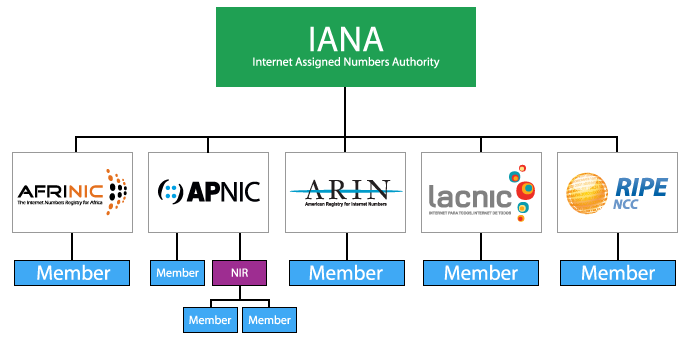
\includegraphics[scale=0.3]{IR-structure-diagram.png}
\caption{Global Structure of the Internet Registry System}
from http://www.ripe.net/internet-coordination/internet-governance/internet-technical-community/the-rir-system
\label{fig:ir_structure_diagram}
\end{figure}

IP addresses are assigned in hierarchical manner as shown in Figure \ref{fig:ir_structure_diagram}. Internet Service Providers obtain allocations of addresses from a Local Internet Registry (LIR), a National Internet Registry (NIR) or from the corresponding Regional Internet Registry (RIR) and in turn they assign IP addresses to end users. IANA's main purpose is to allocate IP addresses from pools of unallocated addresses to the Regional Internet Registries according to their needs. IANA does not make allocation of IP addresses directly to ISPs or users except for allocations of multicast addresses or protocol specific needs. If a RIR requires further IP addresses for allocation, IANA makes an additional allocation to the RIR. There are five RIRs, each one responsible for a specific region: AFRINIC for Africa Region, APNIC for Asia Pacific Region, ARIN for North America Region, LACNIC for Latin America and the Caribbean Regions, RIPE NCC for Europe, Middle East and Central Asia Regions. The five RIRs are represented in Figure \ref{fig:rirs_image}.

\begin{figure}[h!]
\centering
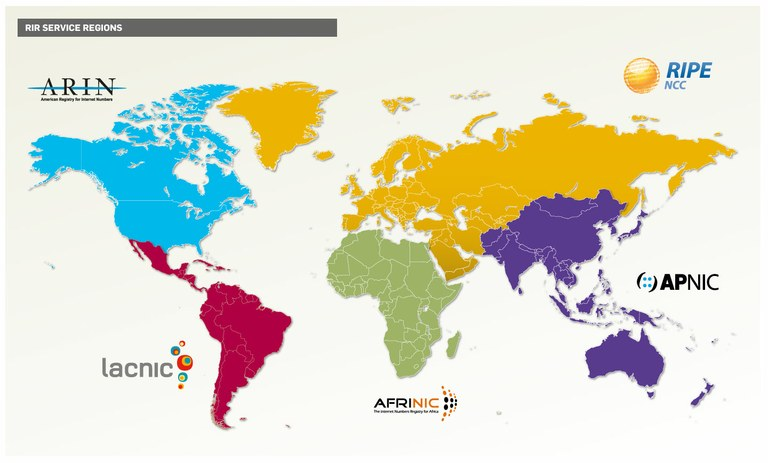
\includegraphics[scale=0.3]{RIR.jpeg}
\caption{Regional Internet Registries Service Regions}
from http://www.ripe.net/internet-coordination/internet-governance/internet-technical-community/the-rir-system
\label{fig:rirs_image}
\end{figure}

\section{Regional Internet Registries}
from http://www.ripe.net/internet-coordination/internet-governance/internet-technical-community/the-rir-system and http://www.ripe.net/lir-services/resource-management/faq/faq-ipv4-address-space


Among the tasks of a RIR are the coordination and representation of the members in its region. RIRs work together in order to develop consistent policies and promote best current practice for the Internet. As mentioned before RIRs are also responsible for allocating and assigning IP addresses within their respective regions. 

Local Internet Registries (LIR) are  established under the authority of a RIR and are responsible for the distribution and registration of address space at a local level. LIRs also ensure that resource allocation policies from RIRs are followed at a local level. LIRs are essentially members of a RIR and are normally operated by Internet Service Providers, but can also be large corportaions, governments and regulators.

from http://meetings.ripe.net/ripe-42/presentations/ripe42-lir-rfc2050/sld002.html using rfc - http://www.rfc-editor.org/rfc/rfc2050.txt and http://www.rfc-editor.org/rfc/rfc7020.txt

The Internet Registry IP Allocation Guidelines were described in RFC 2050, which became obsolete with the introduction of RFC 7020. The objective of this document is to provide information about the Internet Numbers Registry System used in the distribution of globally unique Internet Protocol (IP) address space and autonomous system (AS) numbers and not to propose changes to the current system. Internet number resources are distributed according to three main goals: Allocation Pool Management; Hierarchical Allocation and Registration Accuracy. The goal of Allocation Pool Management is to allocate number resources in accordance to the needs of those running networks, but takink into consideration pool limitations when allocating. This is relevant as the pools from which IP addresses and AS numbers are allocated are finite. Hierarchical Allocation refers to the need of allocating IP addresses in a way that permits their aggregation into a minimum number of routing announcements, in order to ensure continued scaling of the Internet's routing system. The last goal, Registration Accuracy,  requires that a registry of allocations is maintained in order to provide accurate registration information of allocations and ensure uniqueness. This way it is ensured that IP addresses and AS numbers are not allocated to more than one organization.  


   
from http://www.ripe.net/ripe/docs/ripe-606

\section{Border Gateway Protocol}

from paper bgpsurvey.pdf

The internet has a decentralized architecture composed of many interconnected networks, where the end systems are called hosts. At an intermediate level there are routers, which are responsible for selecting the paths that information takes in order to get to the respective end system. The selection of the right path is done by a routing process is determined by routing protocols. These protocols are responsible not only for performing path selectiong, but also to communicate reachability information. A group of IP networks which has a single defined external routing policy is called an Autonomous System (AS) and the process of routing whithin an AS is called intradomain routing, while routing between ASes is called interdomain routing. The de facto protocol used on the Internet for interdomain routing is the Border Gateway Protocol (BGP).
Although BGP has been deployed since the comercialization of the Internet, and version 4 of the protocol has been used for over a decade, it doesn't provide any kind of performance or security guarantees. This limition has already contributed to instabilities and outages \cite{Misdirection} such as a youtube outage caused by Pakistan Telekom \cite{Pakistan}. 

	Thousands ASes make part of the internet and use BGP to exchange information about how to reach blocks of destination IP addresses, which are called IP prefixes. Everytime a new route is available a BGP-speaking router sends an announcement message and when a route no longer exists, it sends a withdrawal message (incremental protocol). BGP is considered a path-vector protocol, because each AS adds its own AS number to the beginning of the AS path before advertising the route to the next AS. Each router will then select one preferred BGP route for each destination prefix. When selecting a route complex policies may be applied which will also decide whether to advertise the route to a neighboring router in another AS.   

	- IP prefixes and AS Numbers
	
	An IP address is a 32-bit number, normally represented in dotted-decimal notation (168.1.2.3), where each of the four octets is represented by a seperate integer. When addresses are assigned to institutions they are blocks of adjacent addresses, which will be represented by the first address of the block and a mask length. The prefix 168.1.2.0/24 contains all the addresses where the first three octets are 168.1.2 and the fourth octet is between 0 and 255, meaning all the addresses between 168.1.2.0 and 168.1.2.255. Allocating addresses in blocks also has the advantage that these blocks can be advertised by routers as a block, instead of having to advertise every IP address, leading to smaller routing tables and less route advertisements. IP prefixes may be contained within another, when that happens an IP router decides to forward a data packet by choosing the longest prefix match according to the destination IP address of that packet. For example, if a router has routing information for two prefixes 168.1.0.0/16 and 168.1.2.0/24 and needs to forward a packet with the destination IP address 168.1.2.3 it will choose the more specific prefix 168.1.2.0/24. 

AS numbers are assigned in a similar manner where from 1 to 64511 are public and have Internet-wide scope. Each number corresponds to only one AS. These numbers can appear in the AS-path attribute of BGP advertisements. Some institutions may not need an unique AS number, for example, if it connects to a single upstream provider that has the responsibility of providing connectivity to the rest of the Internet. In this case the customer may be assigned a private AS number with ranges from 64512 to 65535 for BGP communication with its provider. The provider would then advertise the routes on behalf of the customer. This allows providers to reuse the same private AS number for their customers.

When an AS introduces a destination prefix into the global routing system, by advertising the prefix to its neighboring ASes, it is called the originating AS. In Figure \ref{fig:bgpAdvertisement} we see AS 1 advertising a route for 10.0.0.0/8 with an AS path of "1". When AS 2 receives this advertisement, appends its own AS number to the front of the path and advertises the route with an AS path of "2,1" to the next AS . In the end of this process we see that AS 5 has two diferent paths to the route 10.0.0.0/8 related to its neighbouring ASes.

\begin{figure}[h!]
\centering
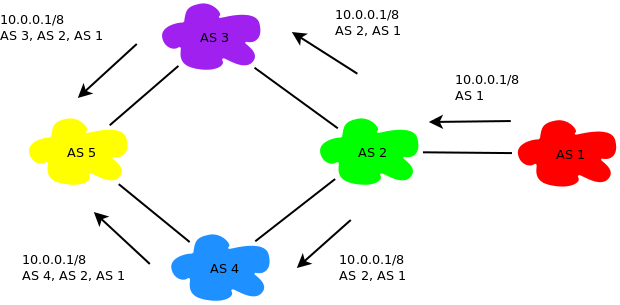
\includegraphics[scale=0.5]{bgpAdvertisement.png}
\caption{BGP Advertisement}
\label{fig:bgpAdvertisement}
\end{figure}

One vulnerability is that BGP does not ensure that a BGP-speaking router making the advertisement for on AS uses the AS number that this AS holds, neither ensures that the AS holds the prefixes it is advertising. As long as the neighboring router accepts the routes, a router can be configured to advertise routes into BGP with any AS number or for any destination prefix, including very small blocks (/30) or address blocks it does not hold. It is possible for the neighboring router to reject such cases, but it needs to be configured for that, meaning that a prior knowledge of acceptable prefixes and prefix lengths is needed. This makes the routing system quite vulnerable to misconfiguration or malicious attacks. The action of an AS advertising an unassigned prefix or belonging to another AS is know as prefix hijacking. When neighboring ASes receive this advertisement they might select the route and direct traffic towards this AS, as well as advertise this BGP route to their own neighbors. In Figure \ref{fig:bgpMaliciousAdvertisement} that AS 1 is advertising route 10.0.0.0/8 and it is the holder of this prefix. If AS 5 starts advertising the route to 10.0.0.0/8 and its neighbours select the shortest path routes, AS 3 and AS 4 will start diverting its traffic with 10.0.0.0/8 destination towards AS 5.

\begin{figure}[h!]
\centering
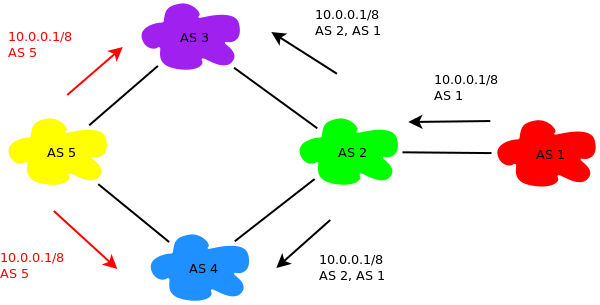
\includegraphics[scale=0.5]{bgpMaliciousAdvertisement.png}
\caption{BGP Malicious Advertisement}
\label{fig:bgpMaliciousAdvertisement}
\end{figure}

In the case that the offending AS just drops all packets destined to the hijacked addresses, the effect is known as a black hole, where the destinations seem unreachable to the parts of the Internet affected by this prefix advertisement. In the case that the AS decides to direct the traffic to hosts under its control the effect can be more severe, as the they can pretend to be the service provided by the hijacked destination. In this situation the traffic received by the AS can be analyzed and sensitive information, such as passwords or credit-card numbers, can fall in the wrong hands. It can also happen that the prefix hijacking is used to analyze the traffic before forwarding it to the correct destination, which would be a breach in the user's privacy. In order for an AS to do such an hijacking attack, it could advertise more specific prefixes then the ones in the original block (e.g., 10.1.128.0/17 and 10.1.0.0/16). This would work because of the longest prefix match rule used by IP routers, that forward packets to the more specific address range. In Figure \ref{fig:bgpDeaggregationAdvertisement} we can see an example. By advertising a more specific prefix (10.0.0.0/9), AS 5 will receive the traffic that had destination to AS 1 .

\begin{figure}[h!]
\centering
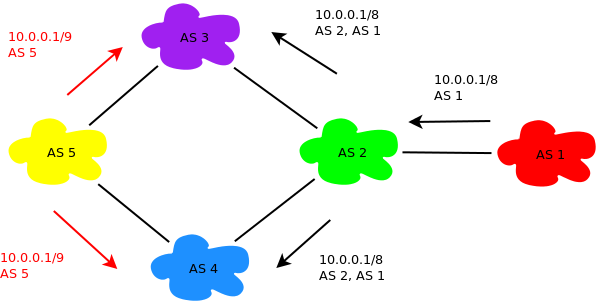
\includegraphics[scale=0.5]{bgpDeaggregationAdvertisement.png}
\caption{BGP Deaggregation Advertisement}
\label{fig:bgpDeaggregationAdvertisement}
\end{figure}


Routers exchange BGP announcement and withdrawal messages by establishing a BGP session with a pair. The BGP session runs over a TCP (Transmission Control Protocol) connection, which provides a reliable way to deliver a stream of ordered bytes, providing error correction and retransmission. BGP neighbors often have a direct physical link at the IP layer, but it can happen that they might have to communicate through an intermediate device. when a BGP session is extablished between ASes it is called an external BGP (eBGP) session, if the session occurs between routers in the same AS it is called an internal BGP (iBGP) session. This last type of sessions happen so that BGP routes learned from neighbors are spread throughout the AS. The communication between two BGP-speaking routers is also vulnerable to attacks, such as attacks against confidentiality, attacks against message integrity and denial-of-service attacks.

Besides being connected through physical links ASes are also bound by business or organizational relationships. An AS can serve as a provider to another organization and therefore there are contractual agreements, which are defined by service level agreements (SLAs). These agreements indicate the quality of service provided or define where the two ASes connect to each other and the traffic they will carry. For such reasons network operators need to be able to influenciate which BGP routes are chosen and which direct traffic will be accepted. For that they need to be able to specify routing policies. With BGP it is possible to enforce routing policies, such as forwarding data just for selected customers by using a number of protocol features. On of such features is the assignment of attribute values in UPDATE messages. BGP-speaking routers choose preferred routes by comparing the route attributes of the possible routes for each destination prefix. When network operators set specific fields in advance they can influenciate how route attributes are set. Among the most important BGP route attributes are:

- Local preference: It is used to override shortest-path routing by prefering other poliy goals and it is propagated inside an AS. It is normally used to prefer routes through a paying customer instead of other neighbors even if the path is longer. This is achieved by assigning a higher local preference value to the router's next-hop AS of the preferred route then to the other next-hops. The same can be applied to direct traffic towards less overcrowded connections, by assigning a high local preference value to this route. 

- AS path length: As mentioned before BGP is a path vector algortihm because each AS adds its AS number to the path before advertising the route. If several routes have the same local-preference value, the route with the smallest AS-path length is chosen, therefore an AS can increase the length of the AS path by adding its AS number to the path multiple times, resulting in a less attractive route to other ASes. This process is known as AS prepending.

- Origin type: Another way to choose a route in case of a tie between several ones is by checking the origin type. A route learned within the AS can be preferred to one learned from the outside, allowing an AS to modify the origin-type attribute to influentiate the choice of a route.

- Multi-Exit Discriminator (MED): It is possible that two neighboring ASes connect to each other at several geographic locations. The MED attribute is used to ensure that traffic is sent to the other AS through the peering location route with the smaller MED. This attribute is typically specified as part of the contract betwwen the ASes.


As seen before BGP routers can can be configured with route attributes in order to influentiate the route that is chosen. This allows to filter received (import policy) and advertised routes (export policy) to its neighbors while choosing where to forward its traffic. The problem is that the way an AS selects routes can be manipulated by sending BGP route announcements with bogus attributes. The AS-path attribute could be truncated to look shorter and therefore more attractive or add additional AS hops at the end. An AS could remove a particular hop from the AS path to modify traffic through certain ASes, or may add an AS number to the AS path so the the target AS would delete ith own AS number thinking it was a loop. An AS could also try to attach MED values to the routes to try to influentiate the route decision. 

from book computer networking

BGP provides each AS ways  to:

- Obtain reachability information from neighboring ASes.
- Propagate the reachability information to all routers internal to the AS
- Determine "good" routes to subnets based on the reachability information and AS policy
- Most importantly, BGP allows each subnet to advertise its existence to the rest of the Internet

In BGP, destinations are not hosts bu CIDRized prefixes, with each prefix representing a subnet or a collection of subnets. BGP peers advertise routes to each other. Two important attributes are AS-PATH and NEXT-HOP:
 - AS-PATH: contains the ASs through which the advertisement for the prefix has passed. When a prefix is passed into an AS, the AS adds its AS number to the AS-PATH attribute.
 -NEXT-HOP: is the router interface that begins the AS-PATH. 



D. Routing Registries
Despite the benefits of protective route filtering,
detecting and disregarding bogus BGP routes is more
challenging when the erroneous information stems from a
misconfiguration or an attack several AS hops away.
Having a shared, global view of Bcorrect[ routing
information would make it much easier to detect invalid
routes. An accurate routing registry [48] of, for example,
prefix ownership, AS-level connectivity, and routing
policies would enable security-conscious ASes to detect
and discard invalid routes. 


\section{Internet Routing Registries}
http://www.nanog.org/meetings/nanog51/presentations/Sunday/NANOG51.Talk34.NANOG51%20IRR%20Tutorial.pdf

from http://www.nsfnet-legacy.org/about.php
http://www.nsf.gov/about/history/nsf0050/internet/launch.htm
http://www.hernandocadett.com/content/stability-and-consistency-internet-wide-network-routing
https://www.nsf.gov/news/news\_summ.jsp?cntn\_id=103050
http://www.merit.edu/research/nsfnet\_article.php
http://www.merit.edu/services/meritradb/history.php

The National Science Foundation inherited the responsability for developing the U.S. Internet from the Advanced Research Projects Agency (ARPA) and the Internet Routing Registry concept goes back to the 1980's and to the National Science Foundation Network (NSFNet).  NSFNET refers to the program sponsored by the National Science Foundation, initiated in 1985, with the purpose of support and promote advanced networking among U.S. research and education institutions. Among its participants were Merit Network, Inc., IBM, MCI, Advanced Network \& Services, Inc., the State of Michigan and many institutions in research and education. As a way to configure the MSFNET's backbone routers, the Policy Routing Database (PRDB) was used since 1989. Merit planned the retirement of PRDB for December 1994, which would be replace by the Routing Arbiter Database (RADB). RADB would then become part of the Internet Routing Registry (IRR) along with RIPE NCC, MCI and other registries. The IRR objective was to be a global public repository of announced routes and routing policy in a common format so that ISPs could use this information to configure their backbone routers and analyze routing policy.

\begin{figure}[h!]
\centering
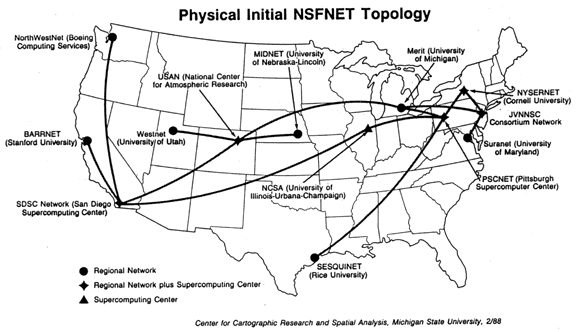
\includegraphics[scale=0.5]{nsfnet_topology.png}
\caption{NSFNET Topology}
from http://www.merit.edu/research/nsfnet.php
\label{fig:nfsnet_image}
\end{figure}

PRDB goal was to maintain information regarding legitimate destination announcements from the various regional networks. This information was very important in order to prevent routing loops. Only after BGP replaced EGP as the inter-domain routing protocol, it became no longer necessary to controll the avoidance of routing loops in such a administratively way. With this change, the information in PRDB turned to be mainly used to gather routing policies, such as path preferences and to generate configuration files for backbone routers.

With the transition of NSFNET to the commercial Internet, the National Science Foundation selected Merit Network and a partner organization to act as Routing Arbiters. The goal of the PRDB would be now to record global routing policy information based on each Autonomous System's policy and RADB comes into the scene. RIPE had pioneered work to record global routing policy information in Europe and the data exchange format described in RIPE-181 (RFC 1786) was adopted as the standar for Internet Routing Registries. This model was also taken by RADB. 

The transition from PRDB presented several problems as the tools used to configure the NSFNET/ANSnet routers were based on PRDB attributes and not RIPE-181. But by December 1994, all the data in PRDB had been converted to RIPE-181-style expressions and on February next year, the RADB had been populated with RIPE-181-style Maintainer and AS Objects. 

\subsubsection{RIPE-181}
from http://www.irr.net/docs/rfc1786.txt


The RFC-1786, which was originally published as a RIPE document (RIPE-181), describes the original database formats that were used by RIPE NCC to store routing policy in its database. As mentioned before RIPE also serves as an allocation registry, which means that its database also contains non-routing oriented objects. 
This documents was also referred as ripe-81++ as it was an update to the original 'ripe-81' proposal for representing and storing routing polices in the RIPE database. Several extensions proposed by Merit Inc. were incorporated into this document and it provided a generalized IP routing policy representation to be used by the Internet routing registries. As it's purpose is to be a general document for Internet routing registries, one can replace the RIPE routing registries by "Regional routing registry".

This document is an important source of information to understand today's Internet registries. 
The Regional routing registries database contains both routing registry and address space allocation registry information. In the begining both informations were combined, but with later it became clear that a separation
of routing information and allocation is desirable. Mainly because in some parts of the world there are different registries for each kind of information and also because often the maintainer of the routing information is not the same as the one of the allocation information.

One of the activities of routing registries is to maintan a databse of IP networks, DNS domains, with information of contact persons and other network management information. The content of this database can be queried using the whois protocol or retrieved as a whole.
The allocation registry contains data about address space allocated to enterprises or delegated to local registries as well as data about the domain name space. 
In the Regional routing registries database the information is stored in form of objects. The types of objects are summarized in table \ref{table:1}.   
   
\begin{table}[h!]
\centering
\begin{tabular}{ | c | c | l | }
\hline
 Registry & Object & Describes \\ \hline
 B & person & contact persons \\
 A & inetnum & IP address space \\
 A & domain & DNS domain \\
 R & auto-num & autonomous system \\
 R & as-macro & a group of autonomous systems \\
 R & community & community \\
 R & route & a route being announced \\
 R & clns & CLNS address space and routing \\
 \hline
\end{tabular}
\caption{Summary of database objects in routing registries}
\label{table:1}
\end{table}

The Registry column gives information to which registry the object belongs to, "A" for allocation registry, "R" for routing registry and "B" for both.

The Objects are represented by attributes value pairs. 
An example of an whois query to retrieve information about network 192.87.45.0 is shown in table \ref{table:2}. Here we can see one inetnum object and two person objects.


\begin{table}[h!]
\centering
\begin{tabular}{  r  l  }
 
 inetnum:  & 	192.87.45.0 - 192.87.45.255 \\
 netname:  & 	OCLC-NET \\
 descr:    &	OCLC \\
 country:  & 	NL \\
 admin-c:  & 	WK1844-RIPE \\
 admin-c:  & 	KDB18-RIPE \\
 tech-c:   & 	WK1844-RIPE \\
 tech-c:   & 	KDB18-RIPE \\
 status:   & 	LEGACY \\
 remarks:  & 	For information on "status:" attribute read https://www.ripe.net/data-tools/db/faq/faq-status-values-legacy-resources \\
 mnt-by:   & 	SN-LIR-MNT \\
 mnt-irt:  & 	irt-SURFcert \\
 source:   & 	RIPE \# Filtered \\
 \\
 person:   & 	Kees van Dobben de Bruyn \\
 address:  & 	Pica Centrum voor Bibliotheekautomatisering \\
 address:  & 	P.O. Box 876 \\
 address:  & 	NL - 2300 AW Leiden \\
 address:  & 	The Netherlands \\
 phone:    & 	+31 71 257174 \\
 fax-no:   & 	+31 71 223119 \\
 nic-hdl:  & 	KDB18-RIPE \\
 mnt-by:   &  	SN-LIR-MNT   \\
 source:   & 	RIPE \# Filtered \\
 \\
 person:   &    Wim Kooreman\\
 address:  &    Pica Centrum voor Bibliotheekautomatisering\\
 address:  &    P.O. Box 876\\
 address:  &    NL - 2300 AW Leiden\\
 address:  &    The Netherlands\\
 phone:    &    +31 71 257257\\
 fax-no:   &    +31 71 223119\\
 nic-hdl:  &    WK1844-RIPE\\
 mnt-by:   &    SN-LIR-MNT\\
 source:   &    RIPE \# Filtered\\
 
\end{tabular}
\caption{Example of whois query response to retrive information about network 192.87.45.0}
\label{table:2}
\end{table}     
        
 
Routing Registry Objects

The most important objects regarding the routing registry are the "aut-num" and the "route" objects. The "aut-num" object describes an autonomous system and the "route" object the route. The "auto-num" object provides contact information for the referred AS and describes its routing policy by identifying the neighboring ASes with which routing information is exchanged. The routing policy is described by identifying what is being announced and what is allowed. The "auto-num" objects provide information how routing information is propagated.
The "route" object describes a single route that is being injected and references the AS that is originating it. In table \ref{table:3} it is shown a "route" object returned from a whois query on network 192.87.45.0. 
The value of the route attribute is a classless address and represents the route being injected into the routing system. The value of the origin attribute is an AS referring to an "aut-num" object, which is the AS injecting this route.
  
\begin{table}[h!]
\centering
\begin{tabular}{  r  l  }

route:    &      192.87.0.0/16\\
descr:    &      SURFnet CIDR Block IV\\
origin:   &      AS1103\\
mnt-by:   &      AS1103-MNT\\
mnt-lower:&      SN-LIR-MNT\\
source:   &      RIPE \# Filtered\\

\end{tabular}
\caption{Example of whois query response to retrive information about network 192.87.45.0 "route" object}
\label{table:3}
\end{table} 


The Autonomous System Object

An Autonomous System (AS) is defined by a group of IP networks which has a single defined external routing policy. An AS has an unique number associated with it. This number is used to identify the AS and to exchange routing information. Routing protocols such as BGP and EGP are used to exchange routing information between ASes.
There are some recommendations that the creation and allocation of an AS should follow such as:
	- It is only needed to create an AS when exchanging routing information 	with other Ases.
	- In a case of customer networks connect to one service provider, the 		IP network should normally be a member of the service providers AS.
    - In the case that a network operator connects to more than one AS with 	different routing policies, it is required for them to have their own 		AS number. 
    - The AS should always try to be populated with as many routes as 		  possible, as long as all routes have the same routing policy
   
An As is represented by an "aut-num" object and "route" objects representing the routes originated by the AS. The "aut-num" object stores administrative information as well as the routing policies of the AS. The origin attributes of the route objects define the set of routes originated by the AS, where each object has only one origin attribute. In table \ref{table:4} it is shown an example of a AS object from a whois query on AS1104.  
    
\# Use this object already new or the old example from the RFC???

\begin{table}[h!]
\centering
\begin{tabular}{  r  l  }

aut-num:    &      	AS1104\\
as-name:    &      	Nikhef\\
descr:   	&     	FOM-Nikhef\\
descr:   	&    	Science Park 105\\
descr:		&   	Amsterdam, 1098 XG\\
descr:   	&	    The Netherlands\\
import:  	&       from AS1103 accept AS1103\\
import:  	&       from AS1139 accept AS1139\\
import:  	&       from AS1888 accept AS1888\\
import:  	&       from AS1126 accept AS1126\\
import:  	&       from AS1124 accept AS1124\\
export:  	&       to AS1103 announce AS1104\\
export:  	&       to AS1139 announce AS1104\\
export:  	&       to AS1888 announce AS1104\\
export:  	&       to AS1126 announce AS1104\\
export:  	&       to AS1124 announce AS1104\\
admin-c: 	&       PK8221-RIPE\\
tech-c:  	&       PK8221-RIPE\\
remarks: 	&       For information on "status:" attribute read https://www.ripe.net/data-tools/db/faq/faq-status-values-legacy-resources\\
status:  	&       LEGACY\\
mnt-by:  	&       AS1104-MNT\\
source:  	&       RIPE \# Filtered\\

\end{tabular}
\caption{Example of whois query response to retrive information about AS1104}
\label{table:4}
\end{table} 

This representation provides a set of routes and a description of administrative details and routing policies. 
        
        
          
          
          
          


	See Appendix A for a complete syntax definition of the "aut-num"
   object.


   It should be noted that this representation provides two things:

       + a set of routes.

       + a description of administrative details and routing policies.

   The set of routes can be used to generate network list based
   configuration information as well as configuration information for
   exterior routing protocols knowing about ASes. This means an AS can
   be defined and is useful even if it does not use routing protocols
   which know about the AS concept.

   Description of routing policies between ASs with multiple connections
   - "interas-in/interas-out"

   The following section is only relevant for ASes which use different
   policies on multiple links to the same neighboring AS. Readers not
   doing this may want to skip this section.

   Description of multiple connections between ASs defines how two ASs
   have chosen to set different policies for the use of each or some of
   the connections between the ASs.  This description is necessary only
   if the ASs are connected in more than one way and the routing policy
   and differs at these two connections.

\chapter{Problem Statement}

from paper THE INTERNET IN TRANSITION: THE STATE OF THE TRANSITION TO IPV6 IN
TODAY'S INTERNET AND OF MEASURES TO SUPPORT THE CONTINUED USE OF
IPV4

Since the 90s that the technical community knows that the use of IPv4 could not scale in a global deployment containing vast concentrations of communicating devices, due to the fact that IPv4 is limited to 4 billion addresses. The technical specification was completed by 1996 and at this time it was initiated a programme to promote the need to transition from IPv4 to IPv6 before the anticipated exhaustion of the IPv4 address pool. The major challenge to achieve this is that IPv6 is not backward compatible with IPv4, meaning that we cannot just replace IPv4 with IPv6. End devices, networks and service delivery points need to be able to support both protocols simultaneously and be able to provide a dual protocol capability before the IPv4 component of the network is taken out of service.     

As illustrated in (reference to paper), the transition to IPv6 is still in an early stage, while the Internet as seen an accelerated growth, with the deployment of more and more connected devices, where mobile devices are playing an important role. This evolution has put pressure on the supply of IPv4, where we assist to a state of IPv4 address exaushtion. At the same time the transition to IPv6, has not been following the rapid deployment. The hope was at the time of the specification was that service providers would prevent the exhaustion of IPv4 addresses and switch to an all-IPv6 network before the pool of IPv4 addresses was depleted. Unfortunately this didn't happen and in February 2011 the pool of IPv4 addresses administred by the Internet Assigned Numbers Authority (IANA) was fully allocated. Two years after, by August 2013, two Regional Internet Registries, APNIC and RIPE, reached a critical low number of managed IPv4 addresses. Nevertheless, the overwhelming majority of end users and services on the Internet continues to rely on IPv4. Because of this the transition to IPv6 was planned as a dual-stack transition, starting from an exclusive model of just using IPv4 to a dual protocol stack mode.

One reason for the delay in deploying IPv6 lies in the supply chain for the Internet's service provider sector. The integration of support for IPv6 in the service provider and customer equipment has taken many years.  

Another reason is the large scale use of Network Address Translation (NAT) by service providers. NAT is placed at the edge of a network and allows multiple devices inside to share a single exterior public address and it has become a common model for Internet service deployment on wired networks. 

The current statistics on address distribution are shown in \ref{fig:rirs_available_ipv4}.

\begin{figure}[h!]
\centering
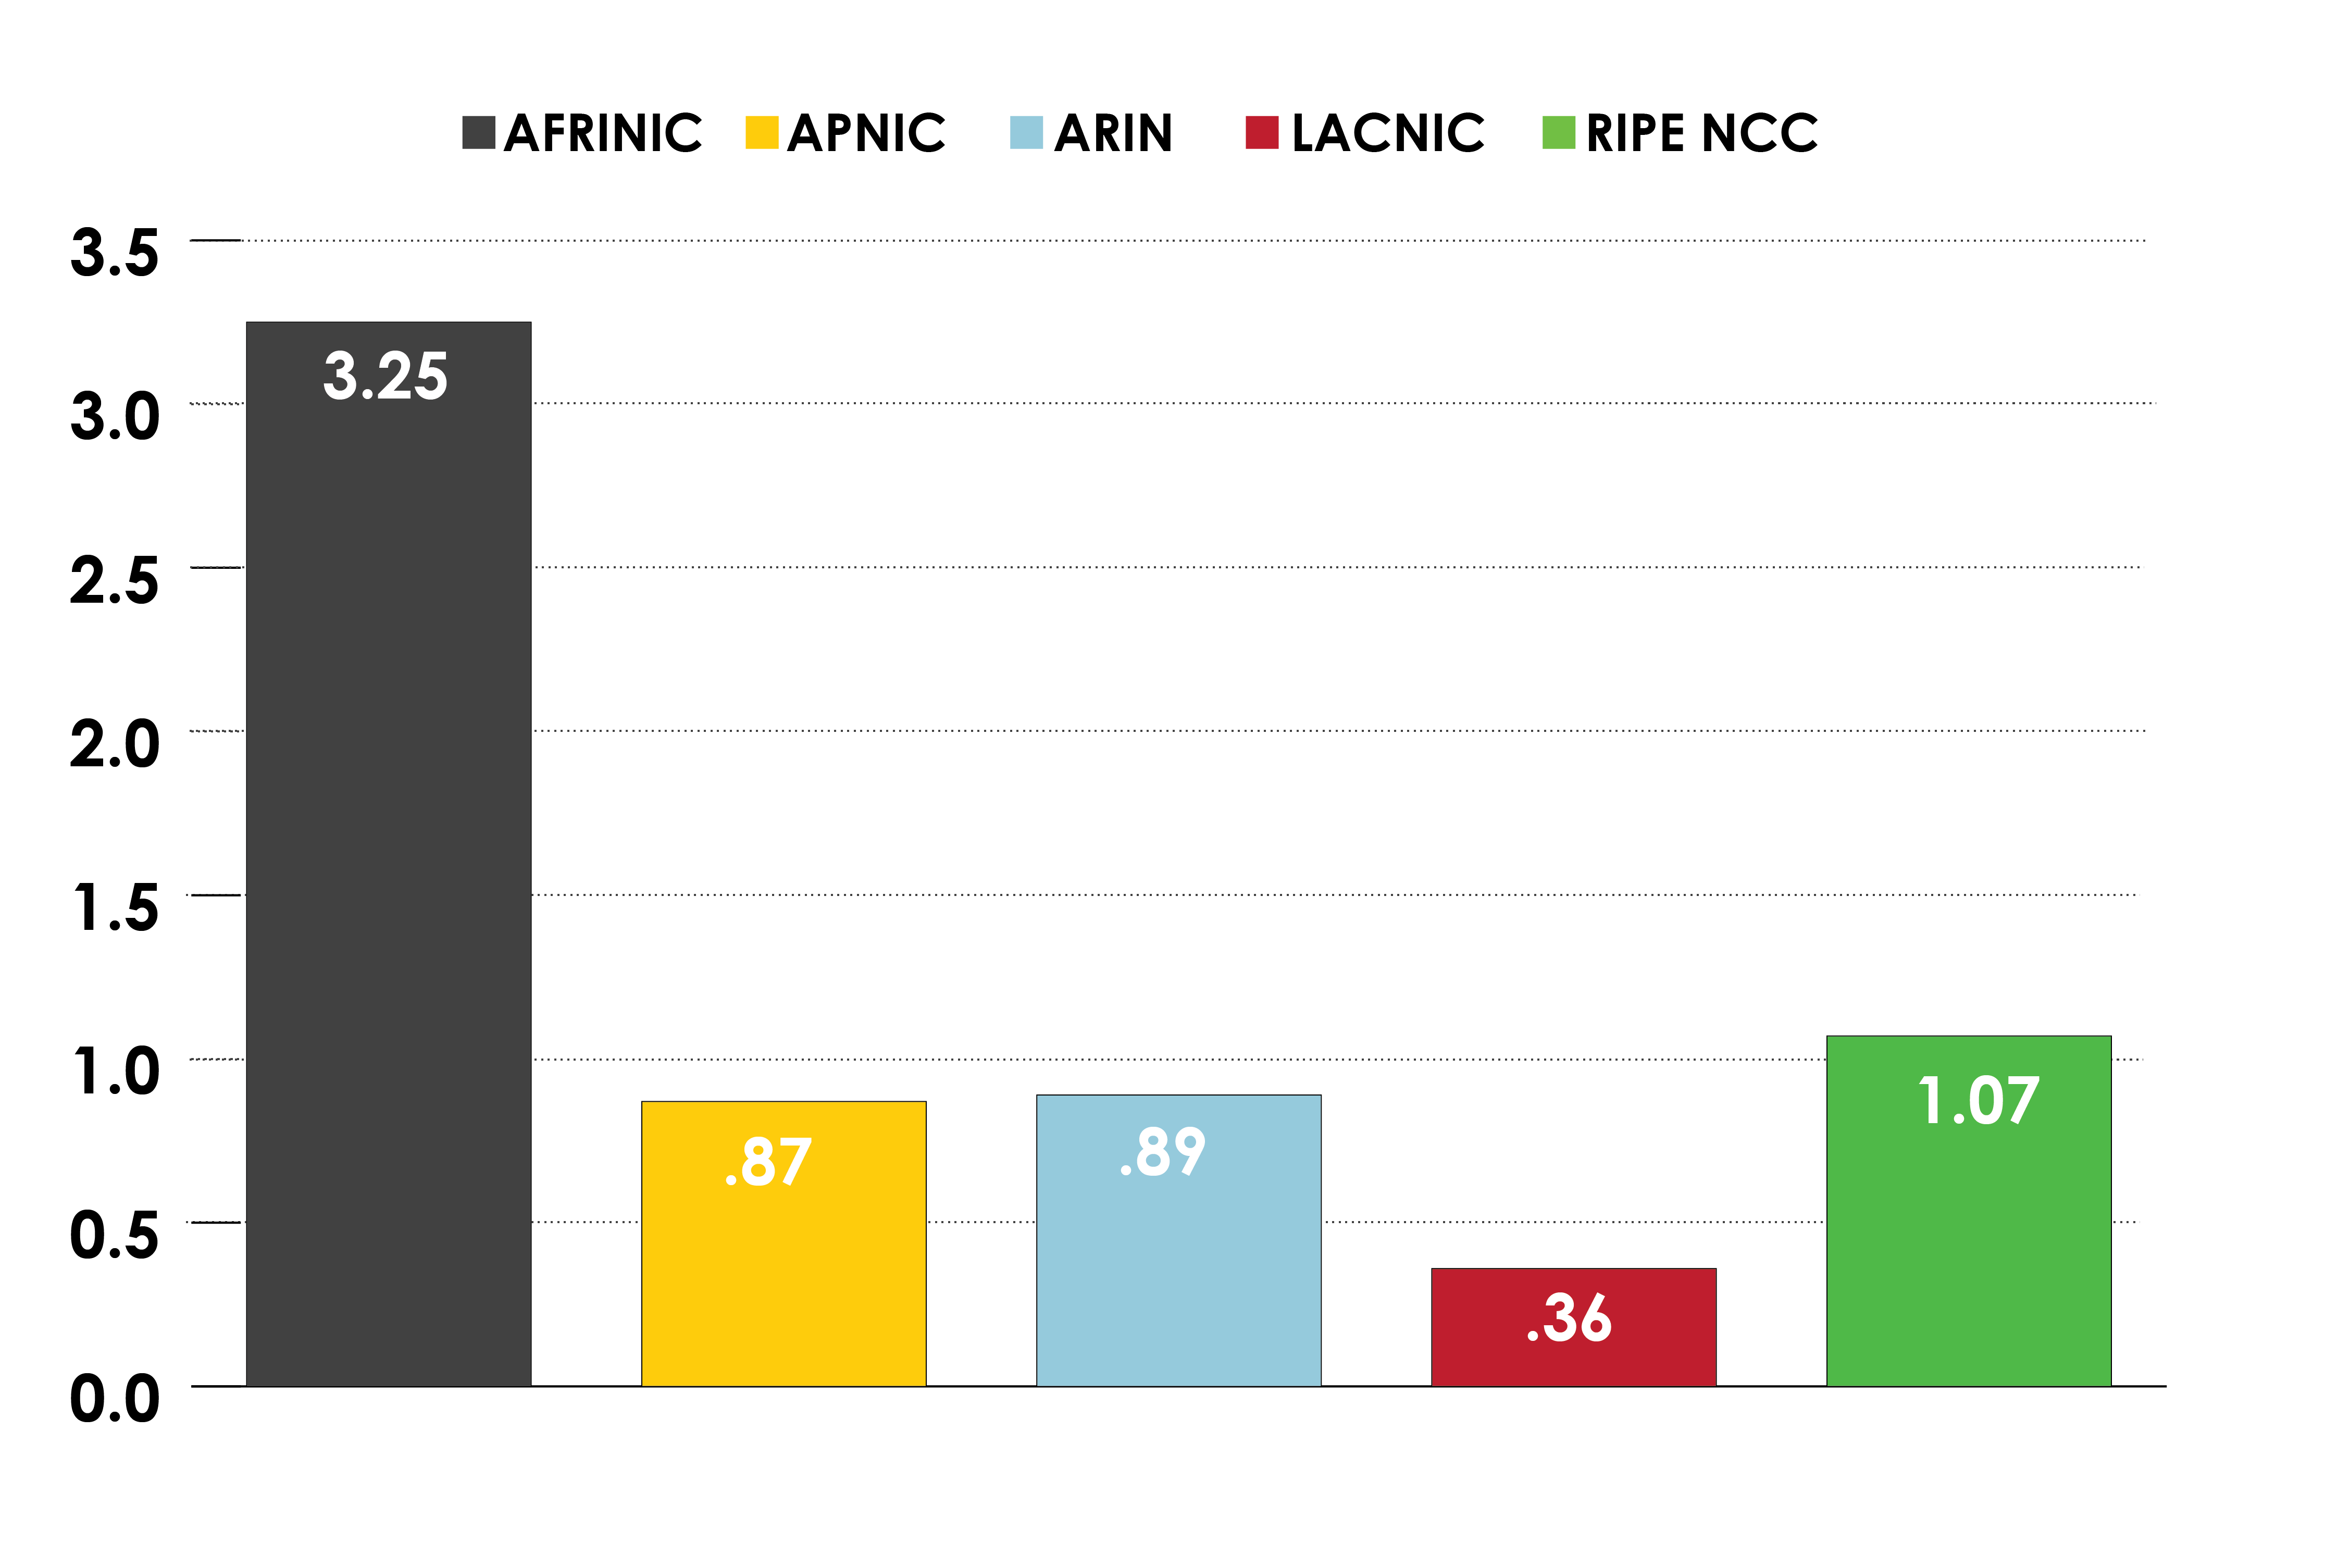
\includegraphics[scale=0.3]{ipv4inRir.png}
\caption{AVAILABLE IPv4 /8s IN EACH RIR}
from https://www.nro.net/wp-content/uploads/NRO\_Q2\_2014-2.pdf June 2014
\label{fig:rirs_available_ipv4}
\end{figure}

We can see that ...

When a local registry or an ISP gets addresses assigned, they can use it in a number of ways. If the address is used for interactions with the public Internet, this address has to be advertised on the routing system. Each individual routing annoucement covers a range of addresses and it doesn't mean that all of these addresses are uniquely assigned to an end device, but normally it is considered that the announcement of a network prefix indicates that the addresses included are being used in some way. Addresses can also be used for some other purpose besides the public Internet, so if one address is not being advertised in the Internet's routing system, it does not a clear indication that it is not being used in an active network.

Due to the fact that many assigned IPv4 addresses might not be being used, it has been discussed within each reagion the possibility of trying to reclaim these addresses. This has several issues for the registries as the agreements between them and the address holders do not oblige the address holders to immediately advertise the assigned addresses on the public Internet and these addresses can also be used in a context where they are not advertised on the public Internet. There is also the case where blocks of addresses were distributed before the creation of the RIR's, called legacy blocks, where there are no formal obligation on the address holder. There has been cases where the responsible RIR has been able to reclaim addresses, specially due to the fact that the address holder didn't fulfill his obligation with respect to the agreement between the parts involved, but the total number of addresses reclaimed had no real impact in the address runout issue.

from paper Scarcity in IP addresses: IPv4 Address Transfer Markets and the Regional Internet Address Registries http://www.internetgovernance.org/wordpress/wp-content/uploads/IPAddress\_TransferMarkets.pdf

In response to the depletion of the IPv4 address space one option could be to allow organizations holding IPv4 addresses to sell address blocks to other organizations interested in bying them. The IP address transfer markets could be a way to extend the life of the IP address space. One major benefit of such a market would be to offer an incentive for address space holders to release unused address resources. An open and legitime transfer market would, as mentioned before, give an incentive to reclaim unused address space, but could also help in a better and accurate registration and administration of address space instead of a gray or black IPv4 address market, which would benefit Internet security.  

from paper Dimensioning the Elephant: An Empirical Analysis of the IPv4 Number Market http://www.internetgovernance.org/wordpress/wp-content/uploads/IPv4marketTPRC20122.pdf

The IP address transfer market can no longer be denied, specially after the deal in which Microsoft bought Notel's address space assets. Either because people believe there should not be a fee for such a resource or because the the transfer market might delay the migration to IPv6, many in the Internet technical community still feel skeptical about it. The truth is that it is difficult to have a comprehensive picture of this market, because the IP number allocations is controlled by five separate regional registries, each one with different databases, disclosure practices and different policies regarding transfers. 

Regarding all this we intend to investigate effects of IPv4 address exhaustion, wether on how it changed the way RIR's are allocating resources or how these resources are being routed.


from paper THE INTERNET IN TRANSITION: THE STATE OF THE TRANSITION TO IPV6 IN
TODAY'S INTERNET AND OF MEASURES TO SUPPORT THE CONTINUED USE OF
IPV4 

Predictions on IPv4 runout
The central pool of IPv4 addresses managed by the IANA functions operator distributed its final
set of address allocations to the RIRs early February 2011. At this stage it continues to manage a set of
address reservations made by the IETF as part of its protocol parameter registry services function, and also
manages a temporary pool of returned so-called legacy addresses prior to their re-distribution to the RIRs.
Of the five RIRs, the first to reach a conclusion of the general address allocation function for
IPv4 addresses was APNIC, on 19 April 2011. Since then, APNIC is operating its continuing IPv4
allocations under a "Last /8 Policy" where each serviced entity may apply for one, and only one, allocation
of up to 1024 addresses. The intent of this policy is to hold onto a small pool of addresses to assist new
entrants in the area of Internet Service Provision to operate in dual-stack mode with some small amount of
IPv4 to service the IPv4 side of their dual-stack needs, with the explicit awareness, noted when the Asia
Pacific regional address policy community was contemplating the adoption of this particular address
policy, that the address block available to each applicant under this policy could be used in conjunction
with IPv4 CGNs so as to allow this very small block of IPv4 addresses to be used in far larger dual-stack
networked environments.15
The second RIR to also run to the end of its general address allocation policies has been the RIPE
NCC, which exhausted its pool on 14 September 2012. The RIPE NCC has also moved into a framework
of a Last /8 Policy with similar constraints in place in APNIC.16
The remaining three RIRs, namely ARIN, LACNIC and AFRINIC, are yet to run out of IPv4
addresses.

In the case of the ARIN registry, it currently holds some 31,267,072 addresses in its local address
pool. In estimating the projected run-out time for this registry it is noted that the model of address
consumption in the region served by this registry changed significantly at the same time as the IANA
registry was depleted in February 2011, which was also the time when this registry changed from a policy
framework that assigned addresses to entities in a quantity that encompassed their planned requirements
for the forthcoming 12 months to one that encompassed only three months of future requirement.

----Mention that in particular we are interested in

\chapter{Related Work}
- Capturing Ghosts: Predicting the Used IPv4 Space by inferring Unobserved Addresses
"The related measure of routed address space has been estimated on prefixes advertised by BGP[Analysis of the IPv4 Address Space Delegation Structure]. Some used ICMP to probe the all allocated internet to infer on the usage." They (their key contribution) used a new statistical capture-recapture technique to estimate the used IPv4 address space from several sources of active and passive measurement data. "Data from nine sources over the past three years suggests 5.8 million used /24 subnets and 740 million used IPv4 addresses. Our CR (capture-recapture) indicates a significantly higher 1.1 billion IPv4 addresses in use across 6.3 million /24 subnets, with usage growing at around 0.5 million /24 subnets and 160 million IPv4 addresses per year." "At this rate all remaining /24 subnets will be used by 2022."

- Analysis of the IPv4 Address Space Delegation Structure
 "Address allocation patterns and its impact on routing table growth were
studied in [17, 23, 29]" 


- A first llok at IPv4 transfer Markets
- A comparative study on IP Prefixe and their Origin ASes in BGP and the IRR
- The Great IPv4 Land Grab: Resource Certification for the IPv4 Grey Market
- Evolution of Internet Address Space Deaggregation: Myths and Reality
- An Analysis of BGP Multiple Origin AS (MOAS) Conflicts


One of the most important source of information is the Potaroo web page \cite{Potaroo}. 
Here we can see statistics regarding IPv4 address space allocation. There is information for each RIR regarding IPv4 address pool status, allocations made and the total span of address space advertised in the BGP routing table over time. It is also possible to obtain the delegation files for each RIR or a joint file.


\chapter{Datasets}

In order to study the advertised IPv4 address space we used BGP table dumps from RouteViews \cite{RouteViews}. This provided us the required raw BGP data for our analysis. As our requirements were just to have a global overview of the prefixes that are being advertised and its origin, to use only this data source would be enough. In case we had to infer about the BGP paths and try to build an internet map, we would certainly have to use more sources (e.g. BGP table dumps from RIPE), but for our analysis this was not necessary as we could obtain a comprehensive view of the global routing system.
We used four collectors, after some previous tests, which would give us the best possible overview of the global system for the entire study period. Some other related work \cite{Address_Space_Deaggregation} used just one collector and still obtained significant results, but we wanted to be on the sure side and decided to use four collectors. 

To be able to study the IPv4 address space allocation history, we used the allocation files \cite{Potaroo} provide by the RIRs.

We used the Whois \cite{Whois} query and response protocol used for querying databases to obtain information about a domain name, an IP address block and an autonomous system. 

We used Merit RADB \cite{RADB} which is a public registry of network routing information as an Internet Registries data source. The choice was to use RADB because its mission is to mirror all Internet Registries  databases to provide the most complete view possible of the entire IRR. 

\section{Data cleaning}
The RouteViews collectors contains the bgp information provided by the peer ASes. For our case study, most of the information is redundant. As we intend to analyze the prefixes that are being advertised and who is advertising them (origin), this information will be provided by most of the peer Ases. The first step to arrange our data and remove redundant information was to identify the most relevant peers. These would be the ones that would provide us the most complete view of the entire internet reagarding the number of prefixes that are advertising and how reliable they were throughout the entire time period of our analises. In \ref{fig:peers1} it is shown all the information gathered from 2001 until 2014. 

\begin{figure}[h!]
\centering
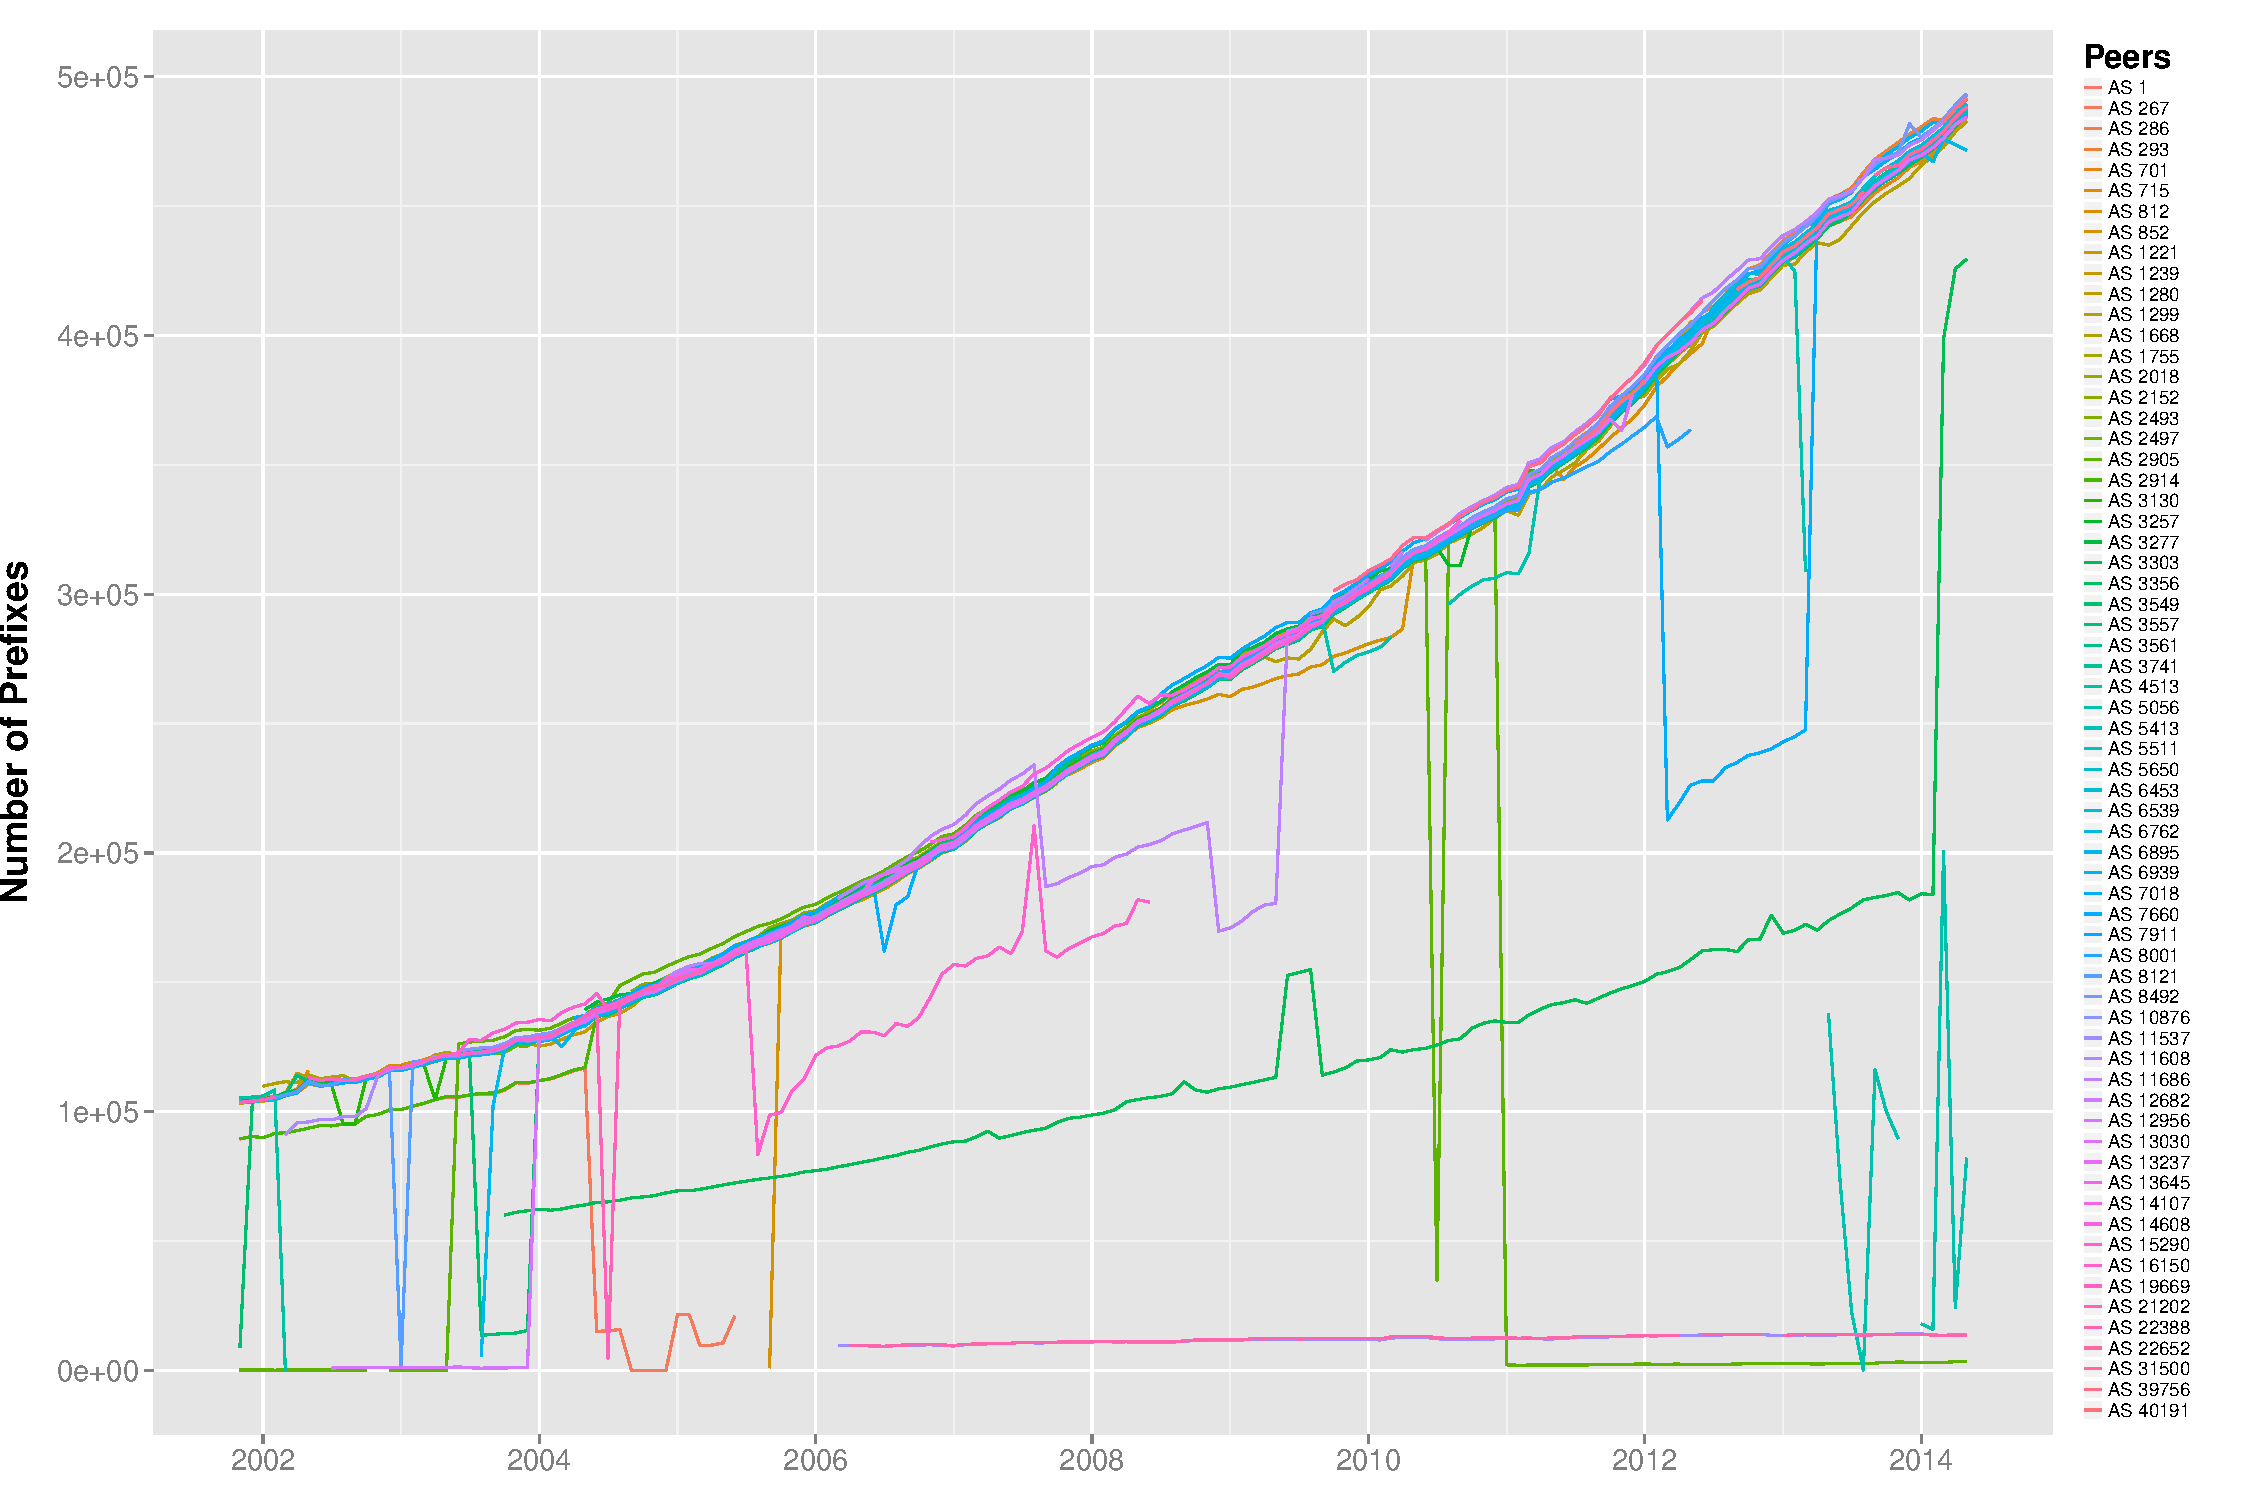
\includegraphics[scale=0.4]{peers1.pdf}
\caption{Peers 1}
\label{fig:peers1}
\end{figure}

It is possible to see that a great number of peers provide less information than others and also that a high number of peers don't provide information whitout breaks throughout the time period. We then procceeded to remove all the peers that delivered a lower number of advertised prefixes or that didn't deliver information at a determined point in time. The result is shown in \ref{fig:peers2}.  

\begin{figure}[h!]
\centering
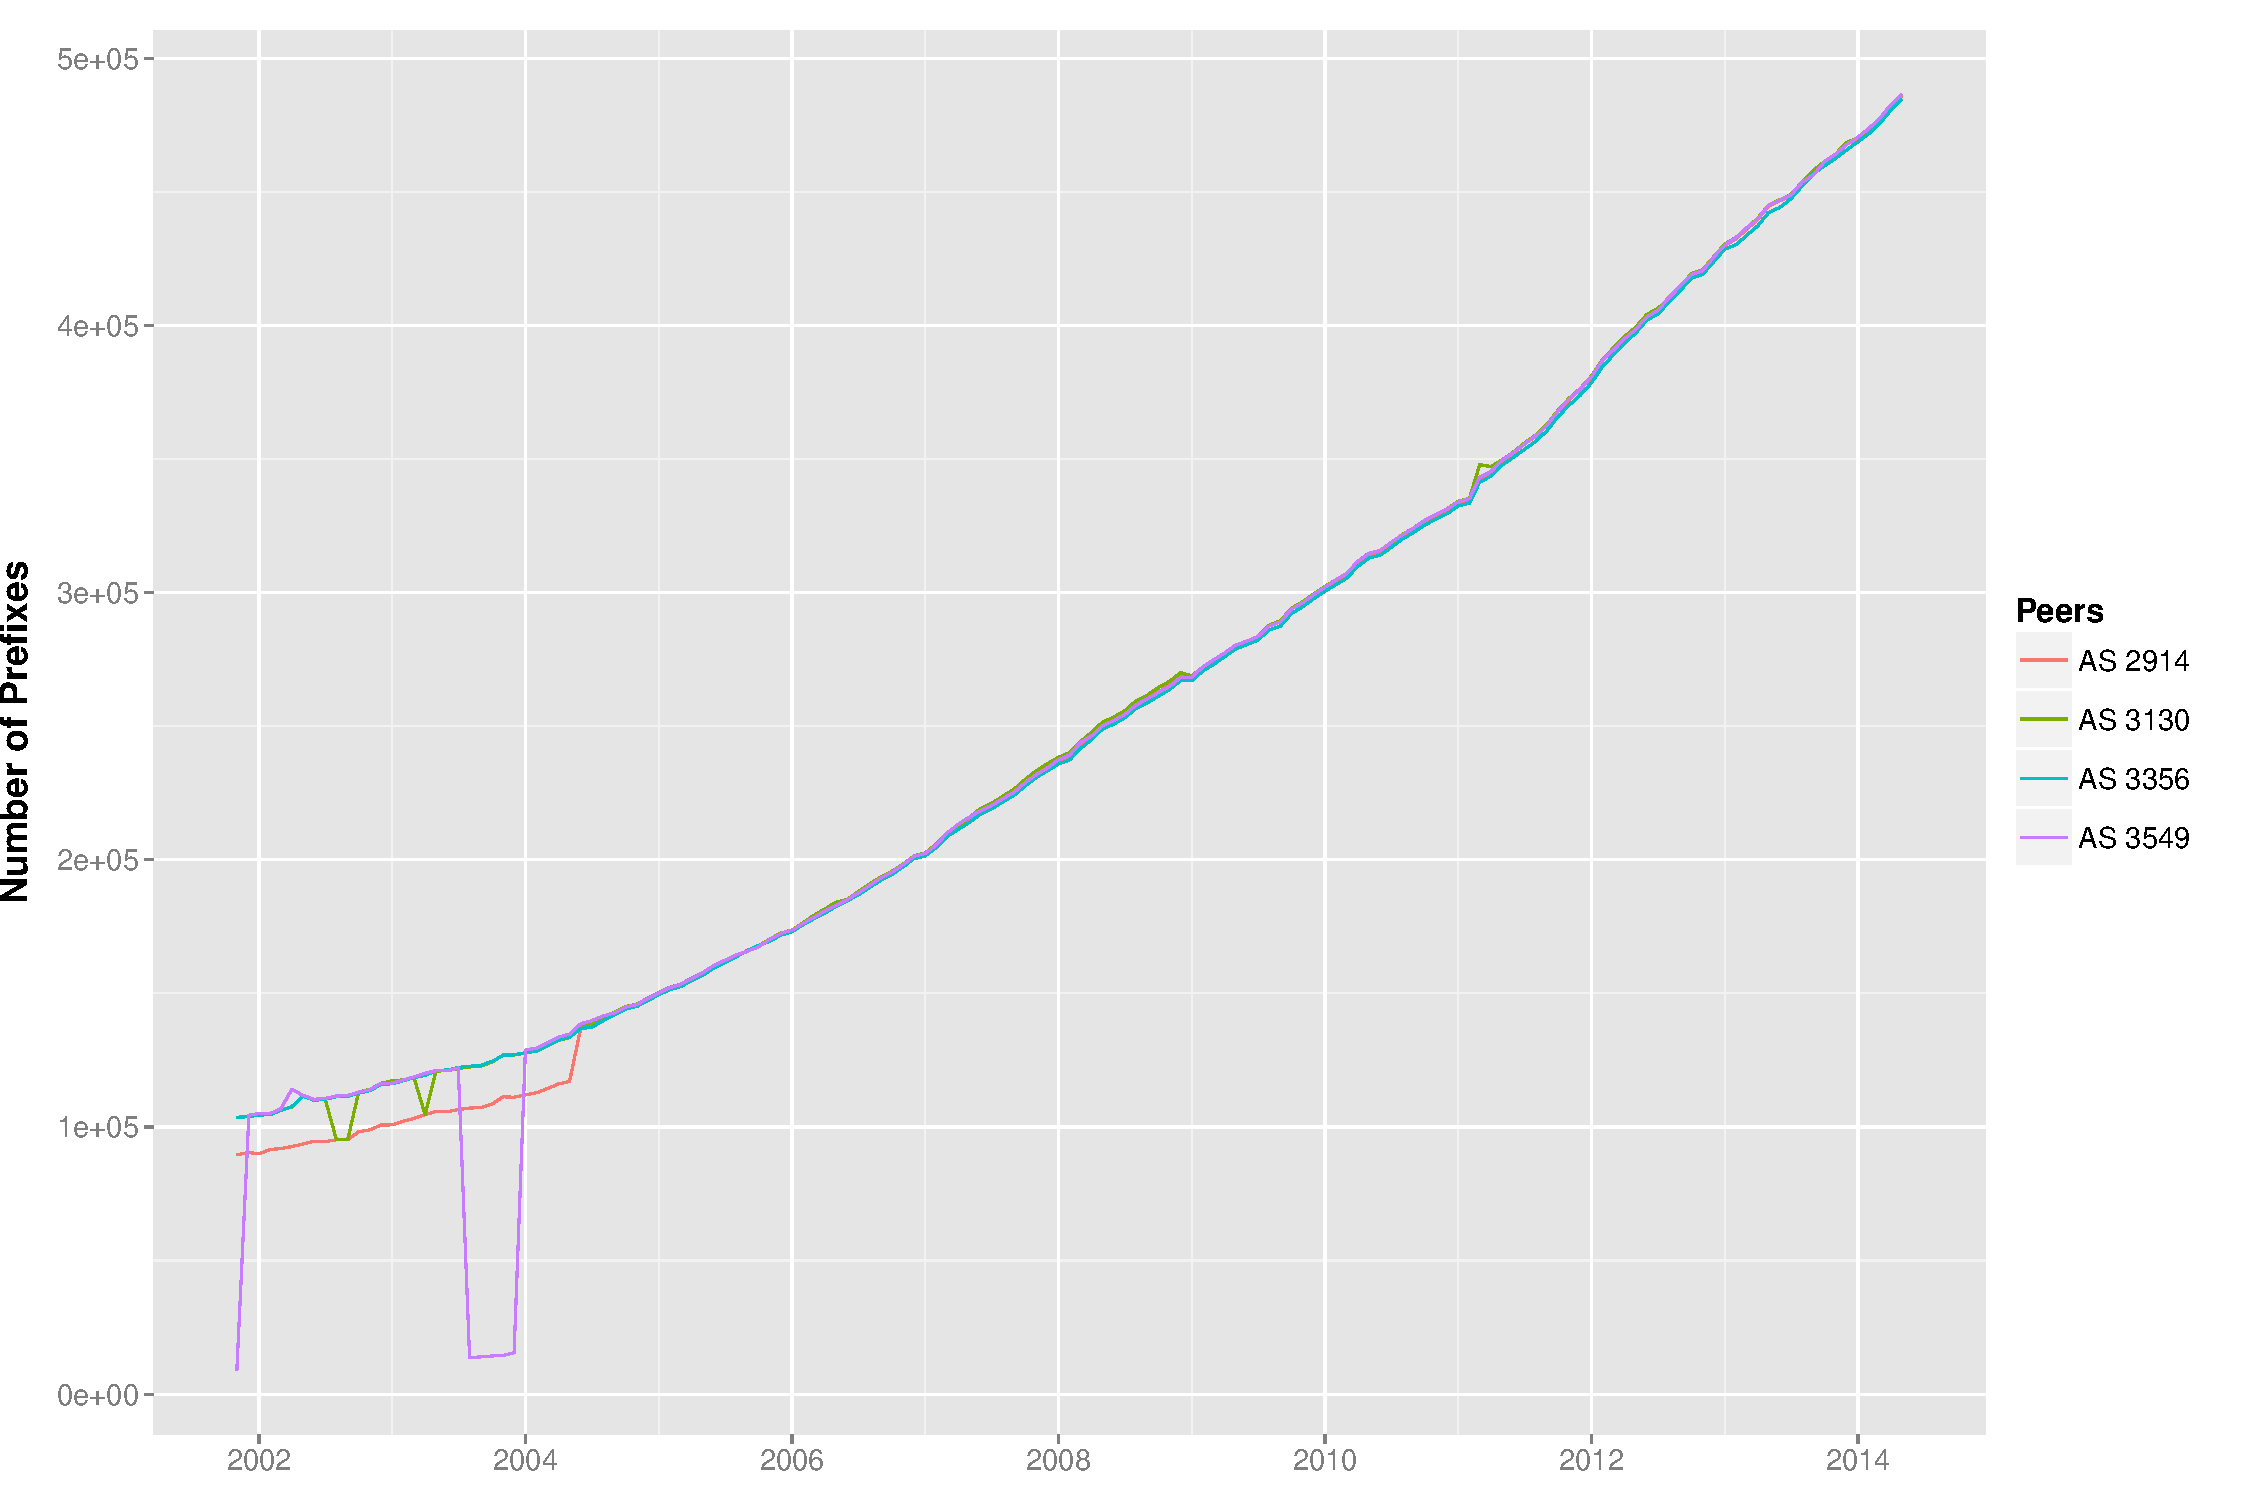
\includegraphics[scale=0.4]{peers2.pdf}
\caption{Peers 2}
\label{fig:peers2}
\end{figure}

By doing this we reduced drastically the amount of data that would have to be analyzed and at the same time we would have a dataset capable of ensuring the best possible data quality. 

\chapter{Results}



\begin{figure}[h!]
\centering
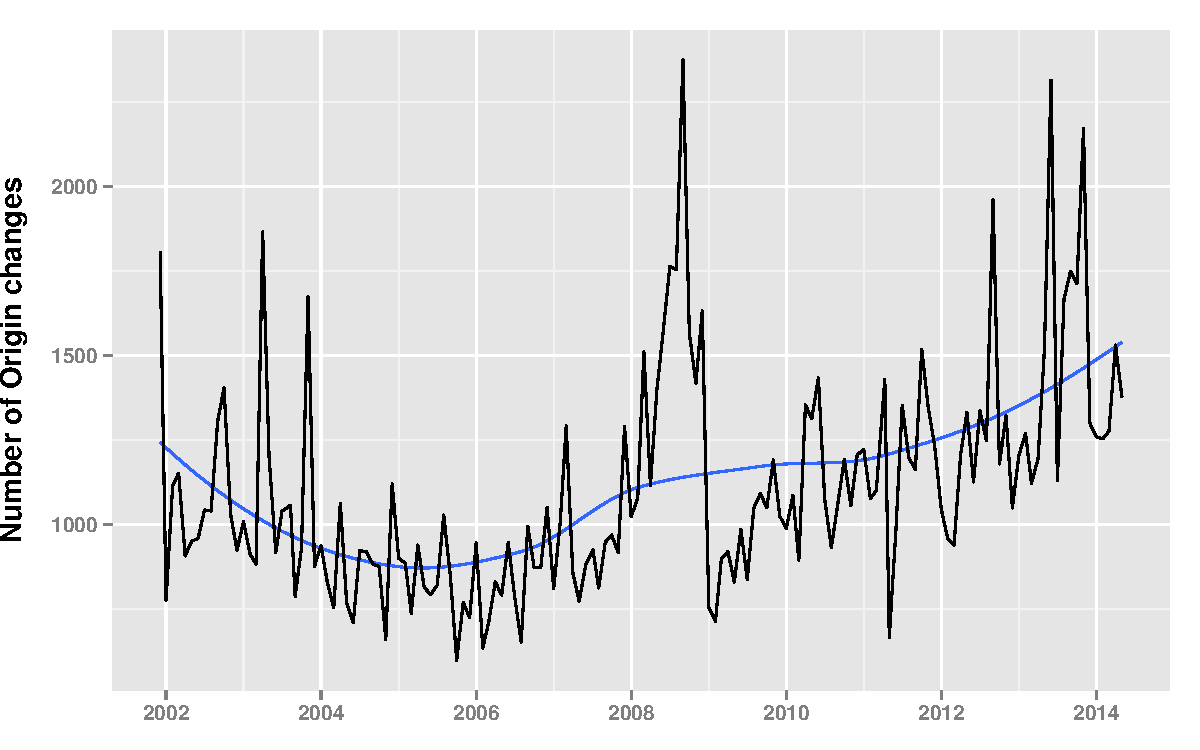
\includegraphics[scale=0.4]{comparePrefixes.pdf}
\caption{comparePrefixes}
\label{fig:comparePrefixes}
\end{figure}

\begin{figure}[h!]
\centering
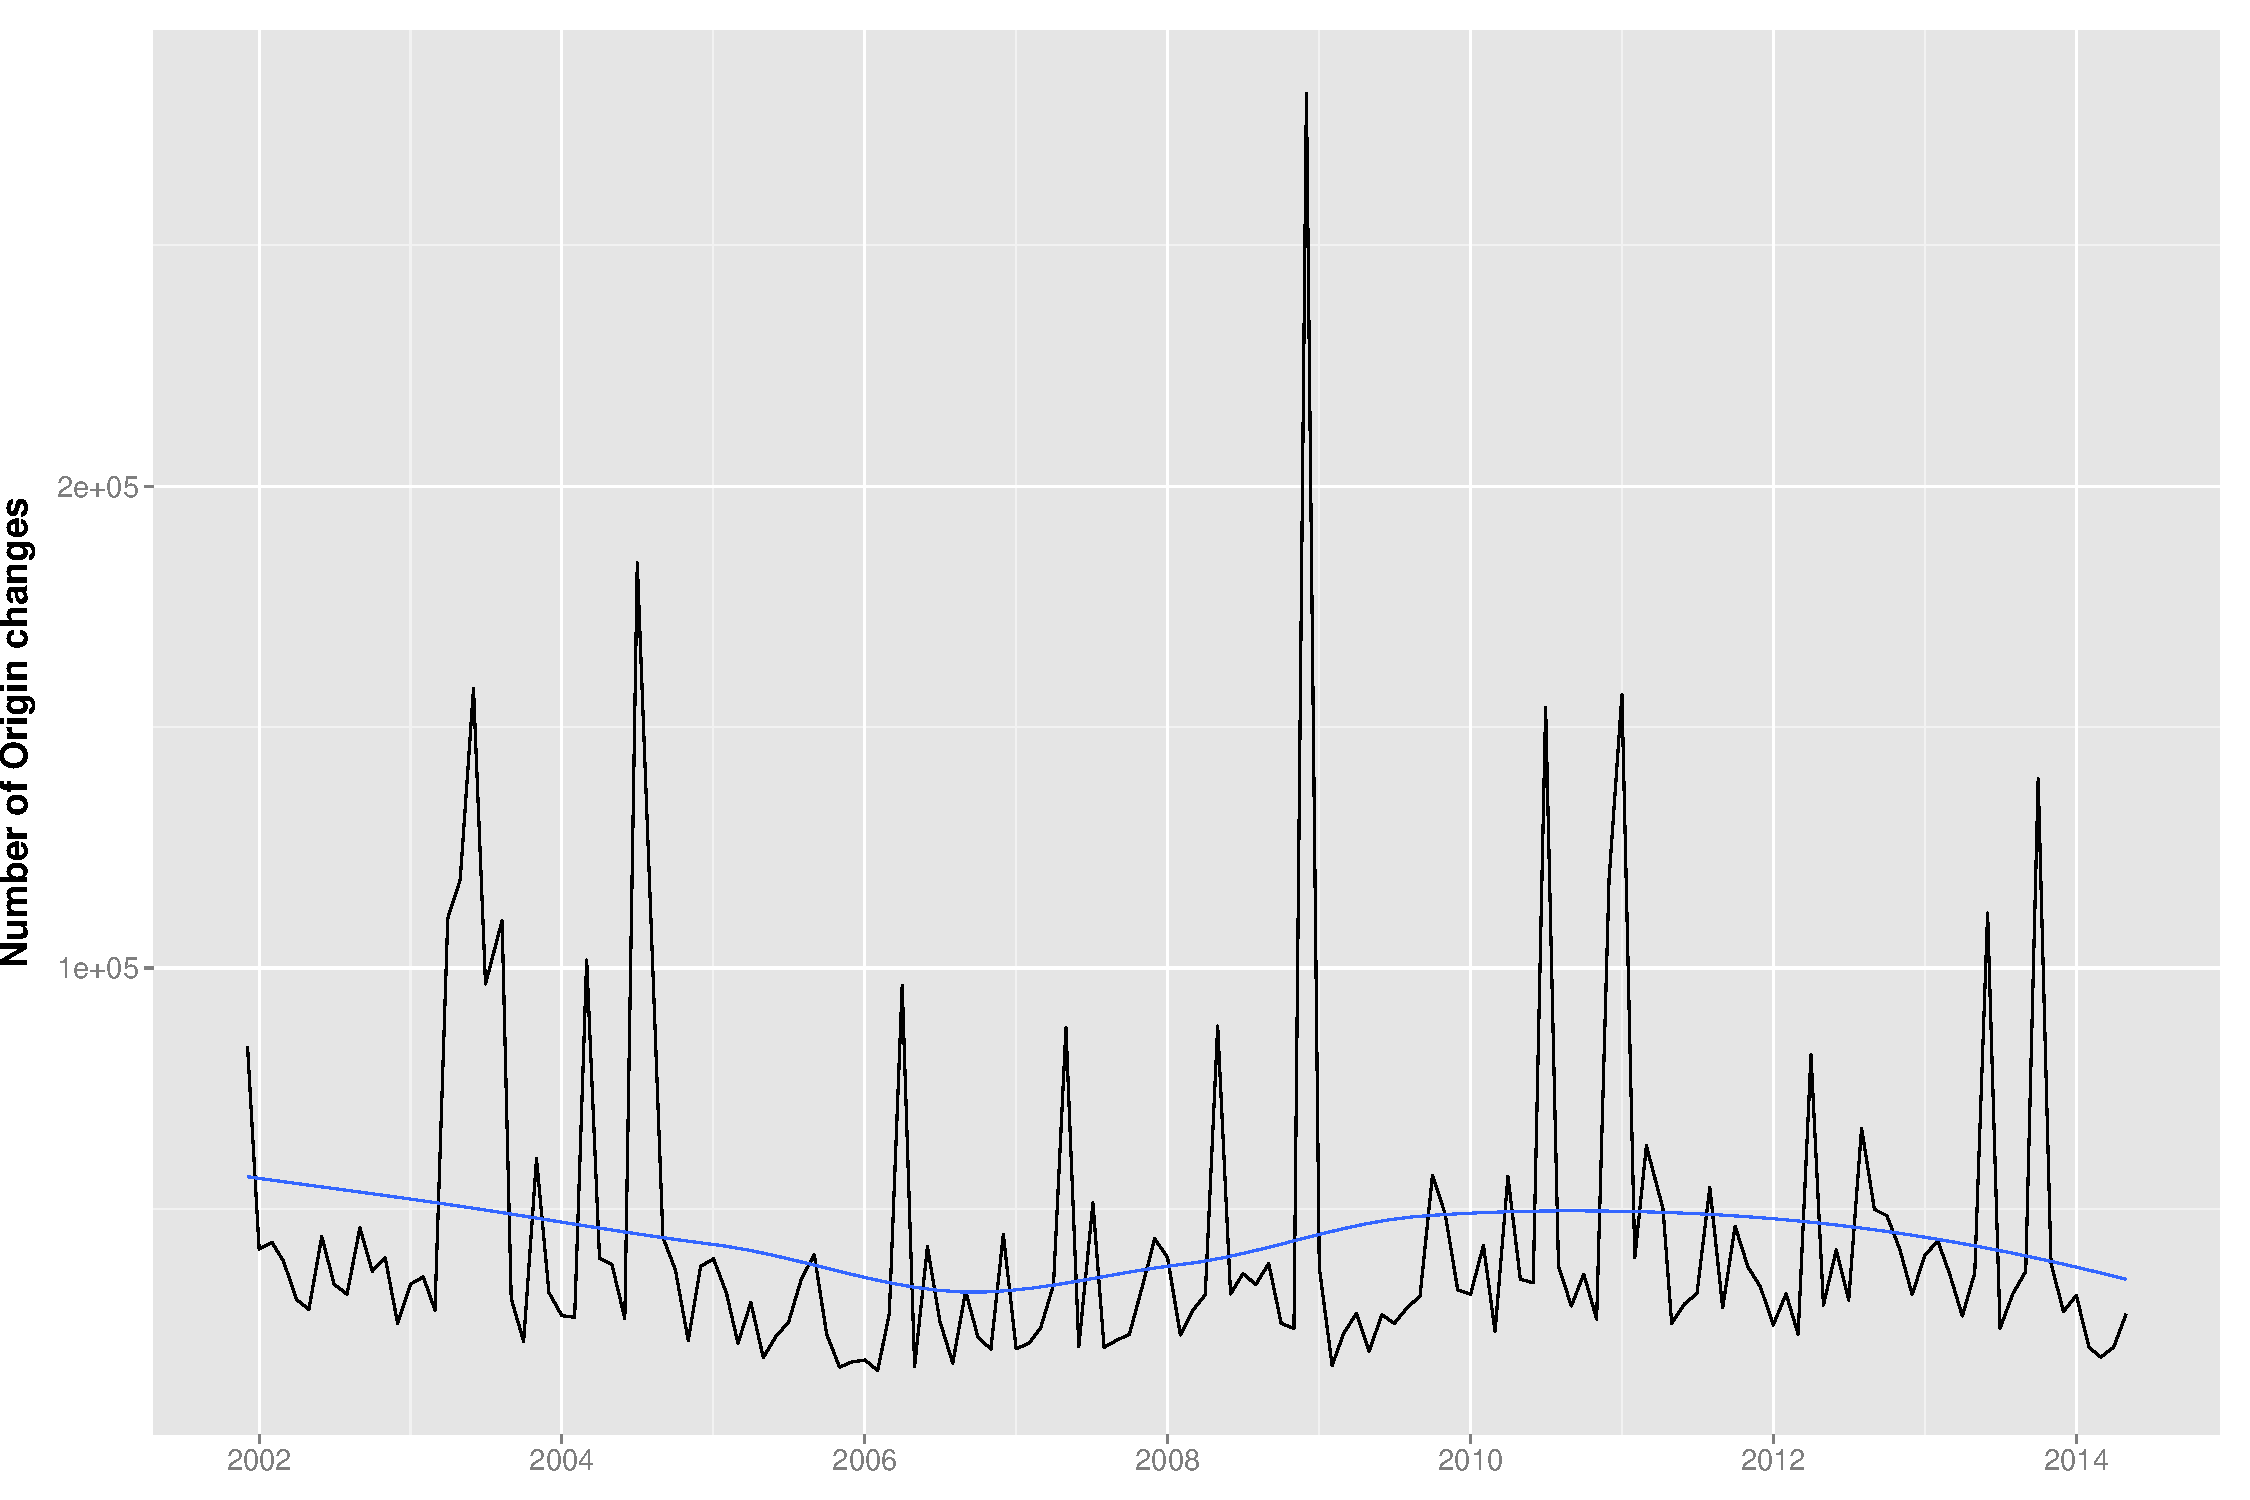
\includegraphics[scale=0.4]{comparePrefixes_24.pdf}
\caption{comparePrefixes24}
\label{fig:comparePrefixes_24}
\end{figure}

\begin{figure}[h!]
\centering
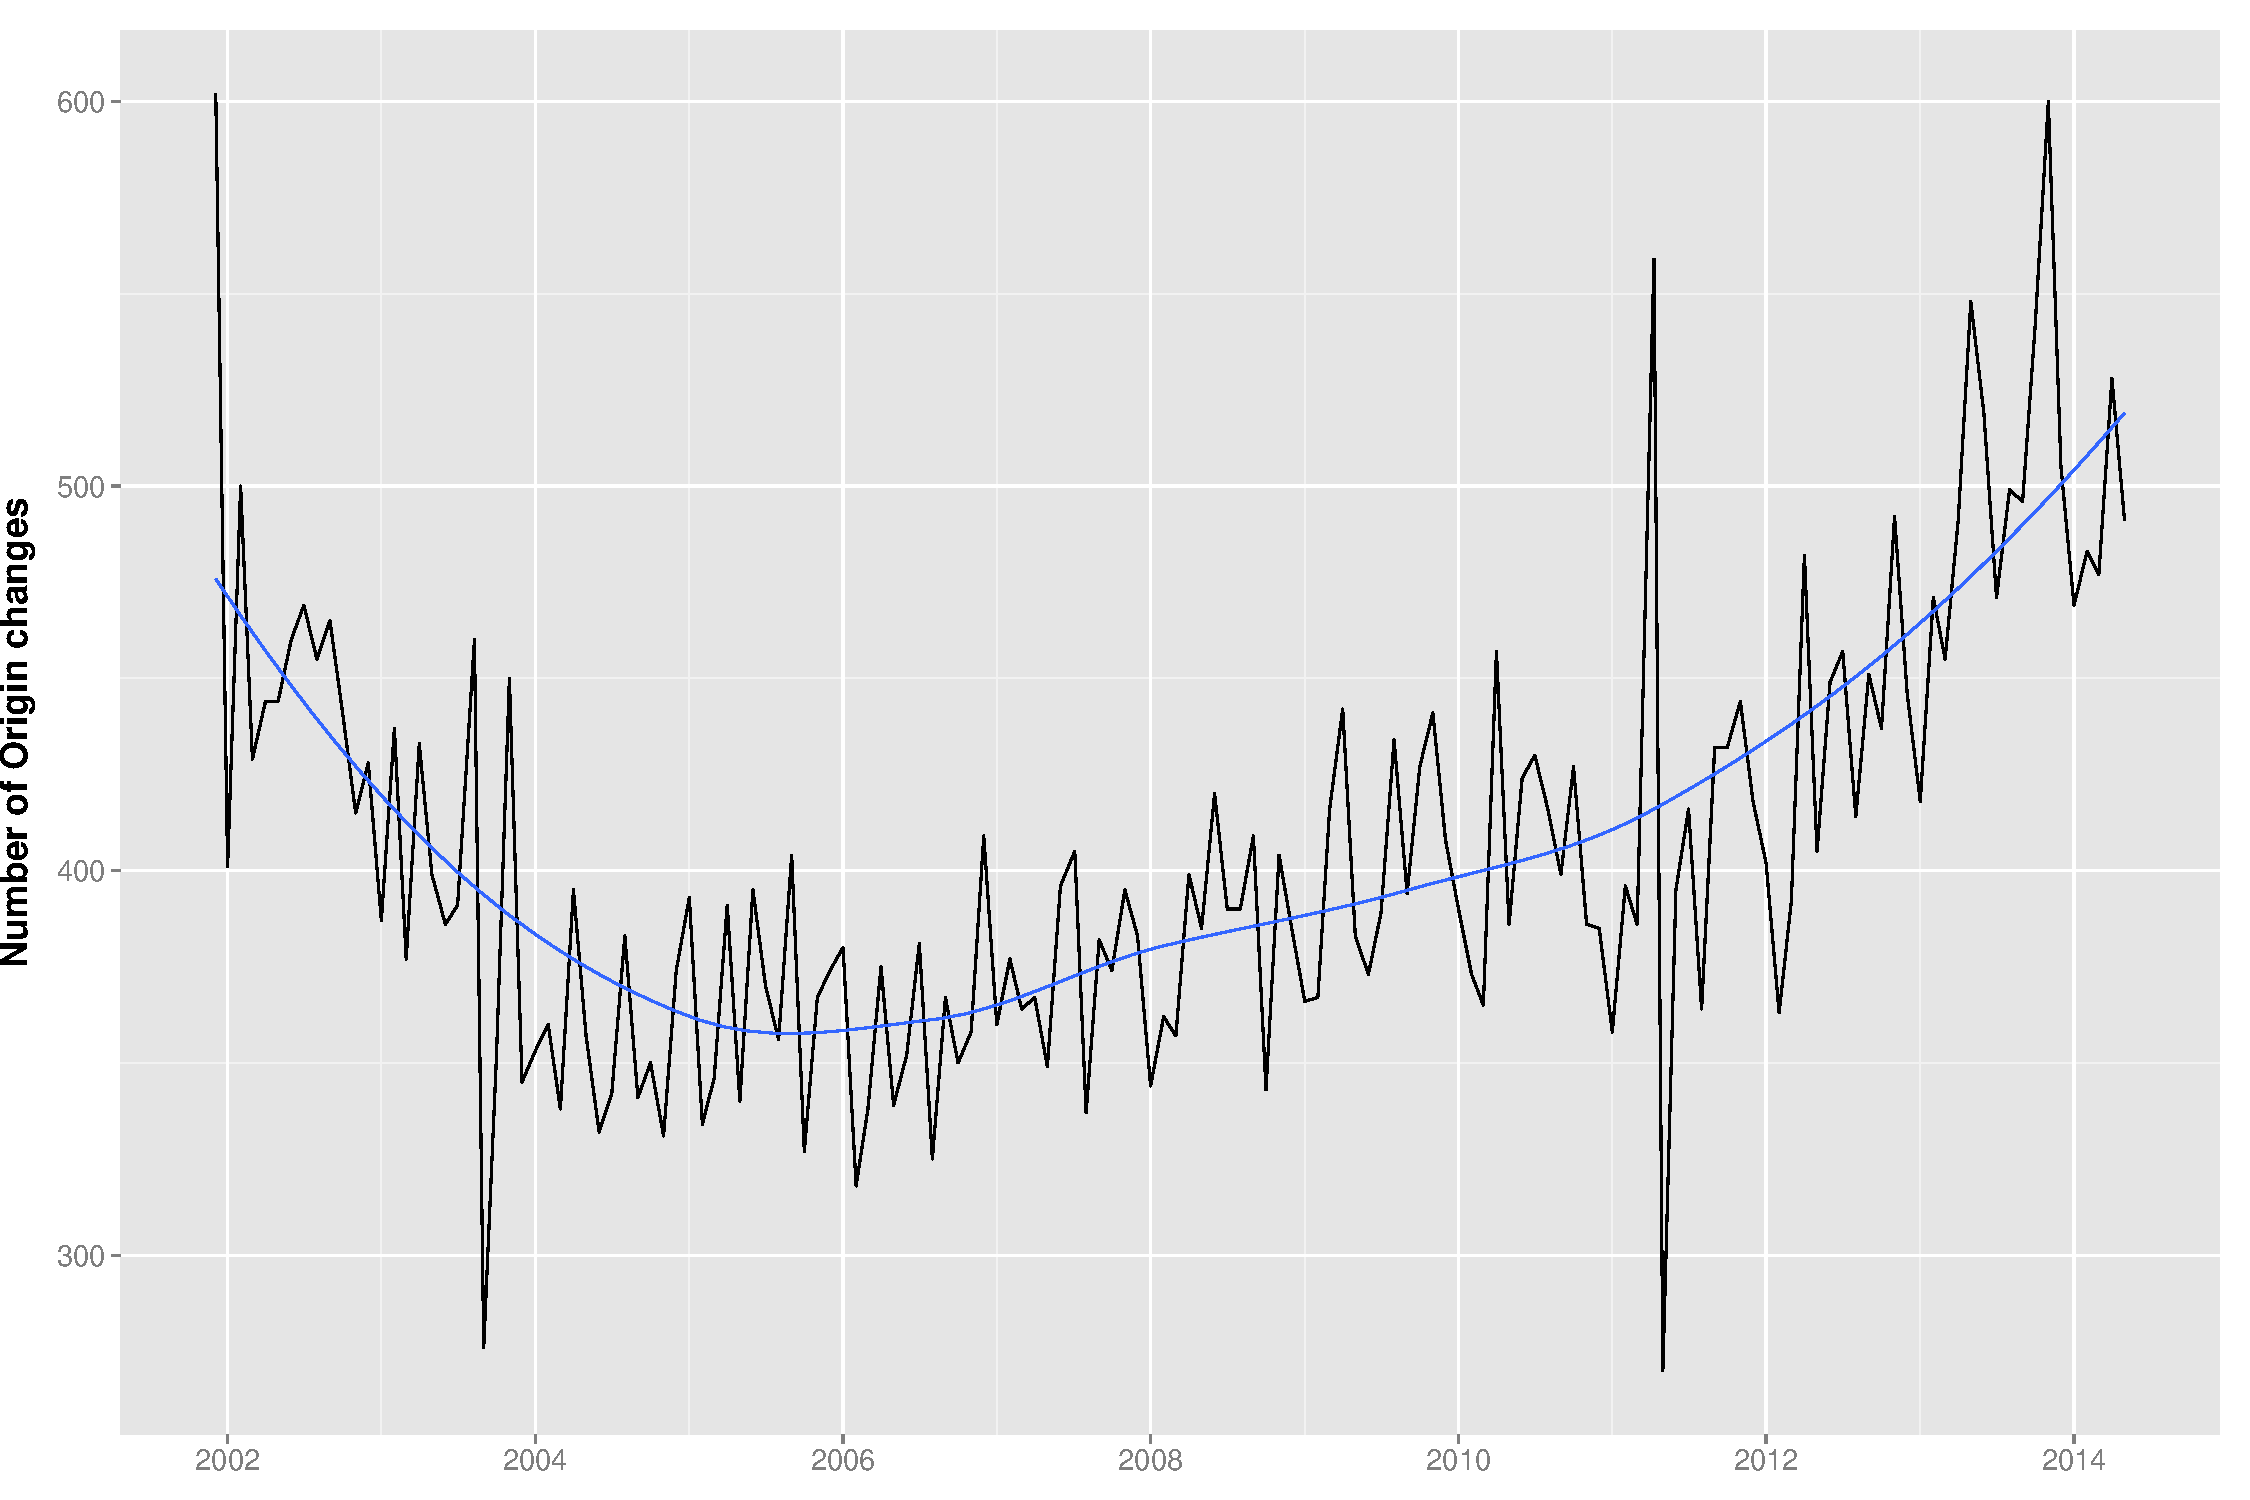
\includegraphics[scale=0.4]{compareAggregation.pdf}
\caption{compareAggregation}
\label{fig:compareAggregation}
\end{figure}

\begin{figure}[h!]
\centering
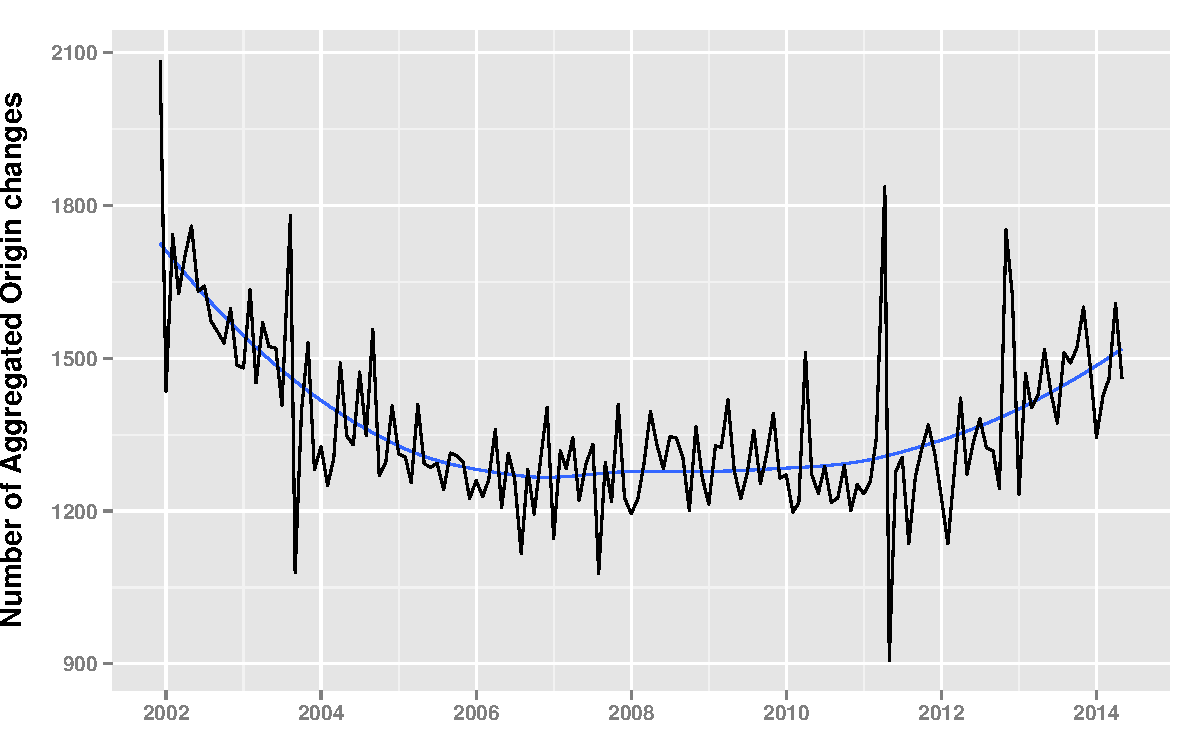
\includegraphics[scale=0.4]{compareAggregation_24.pdf}
\caption{compareAggregation24}
\label{fig:compareAggregation24}
\end{figure}

\begin{figure}[h!]
\centering
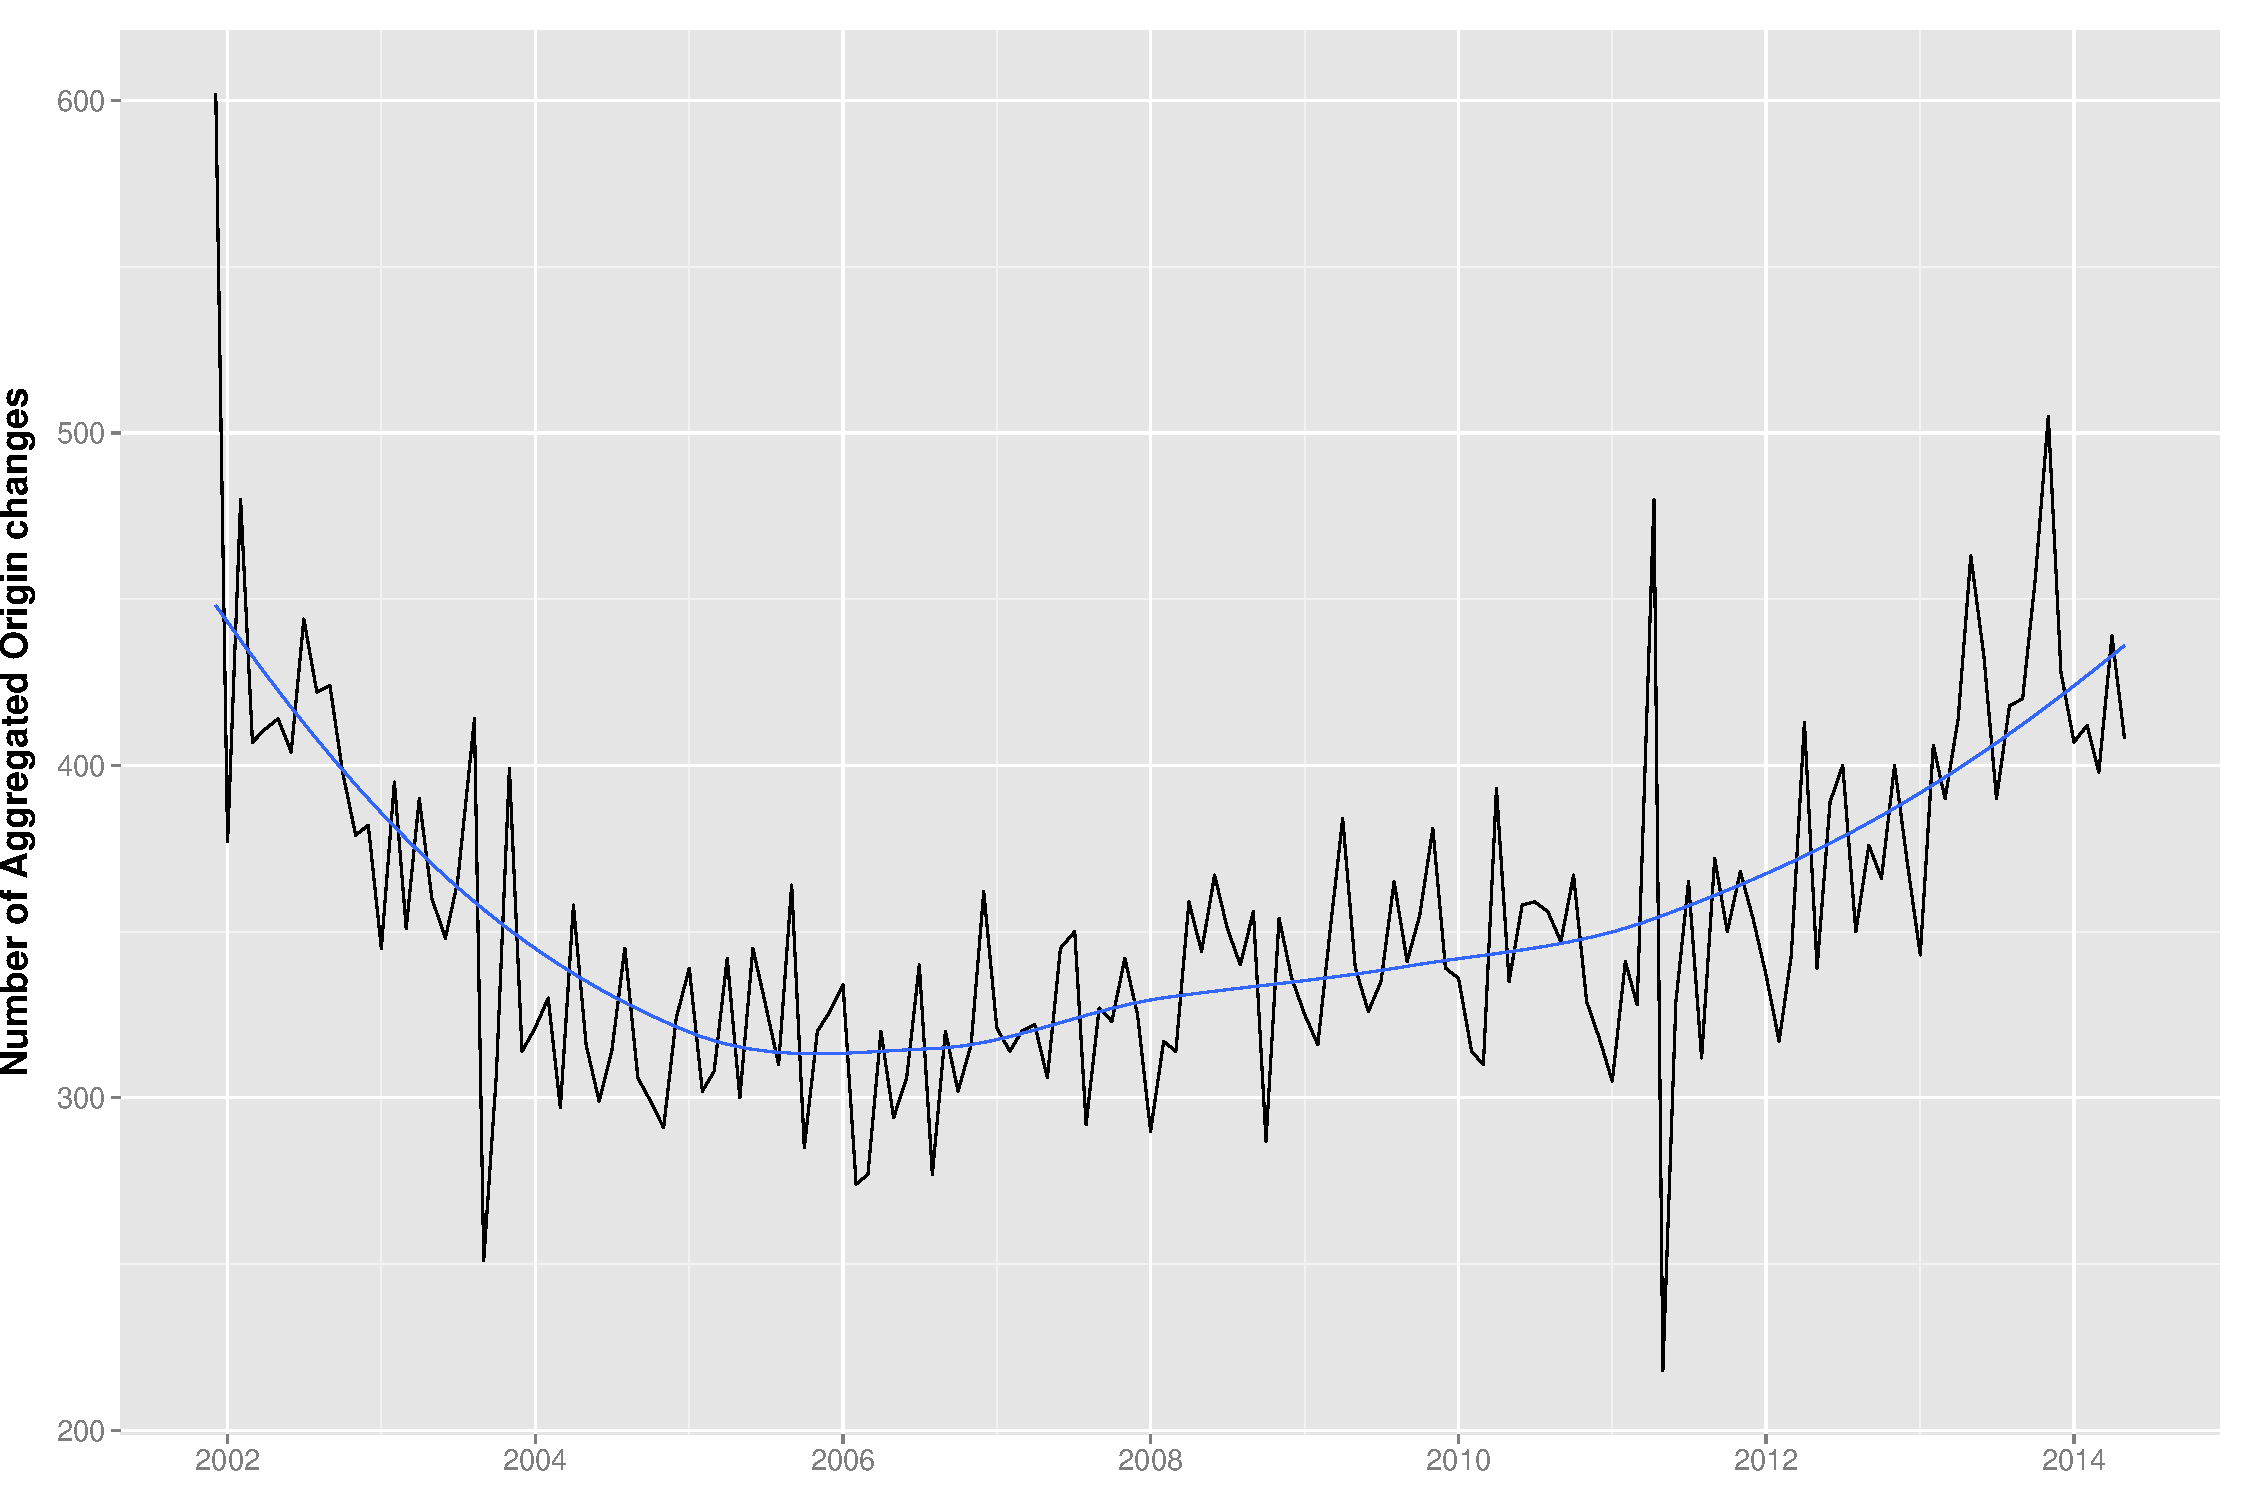
\includegraphics[scale=0.4]{compareAggregationCycles.pdf}
\caption{compareAggregationCycles}
\label{fig:compareAggregationCycles}
\end{figure}

\begin{figure}[h!]
\centering
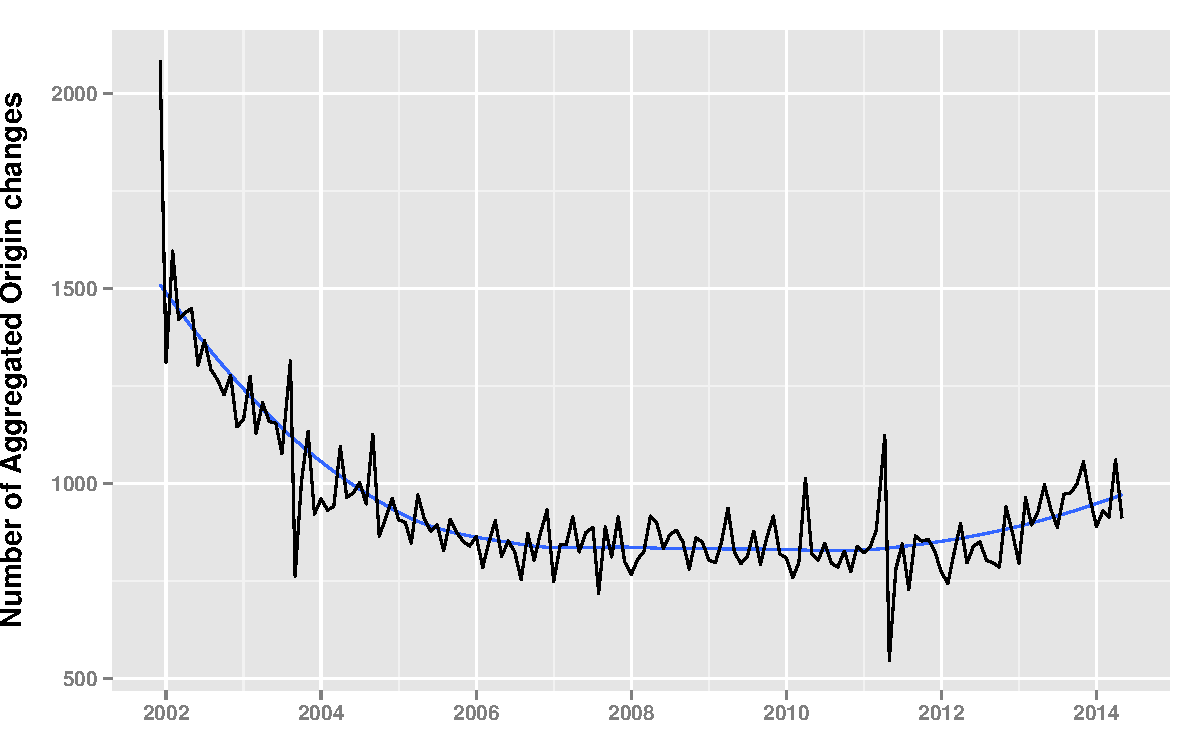
\includegraphics[scale=0.4]{compareAggregationCycles_24.pdf}
\caption{compareAggregationCycles24}
\label{fig:compareAggregationCycles24}
\end{figure}

\begin{figure}[h!]
\centering
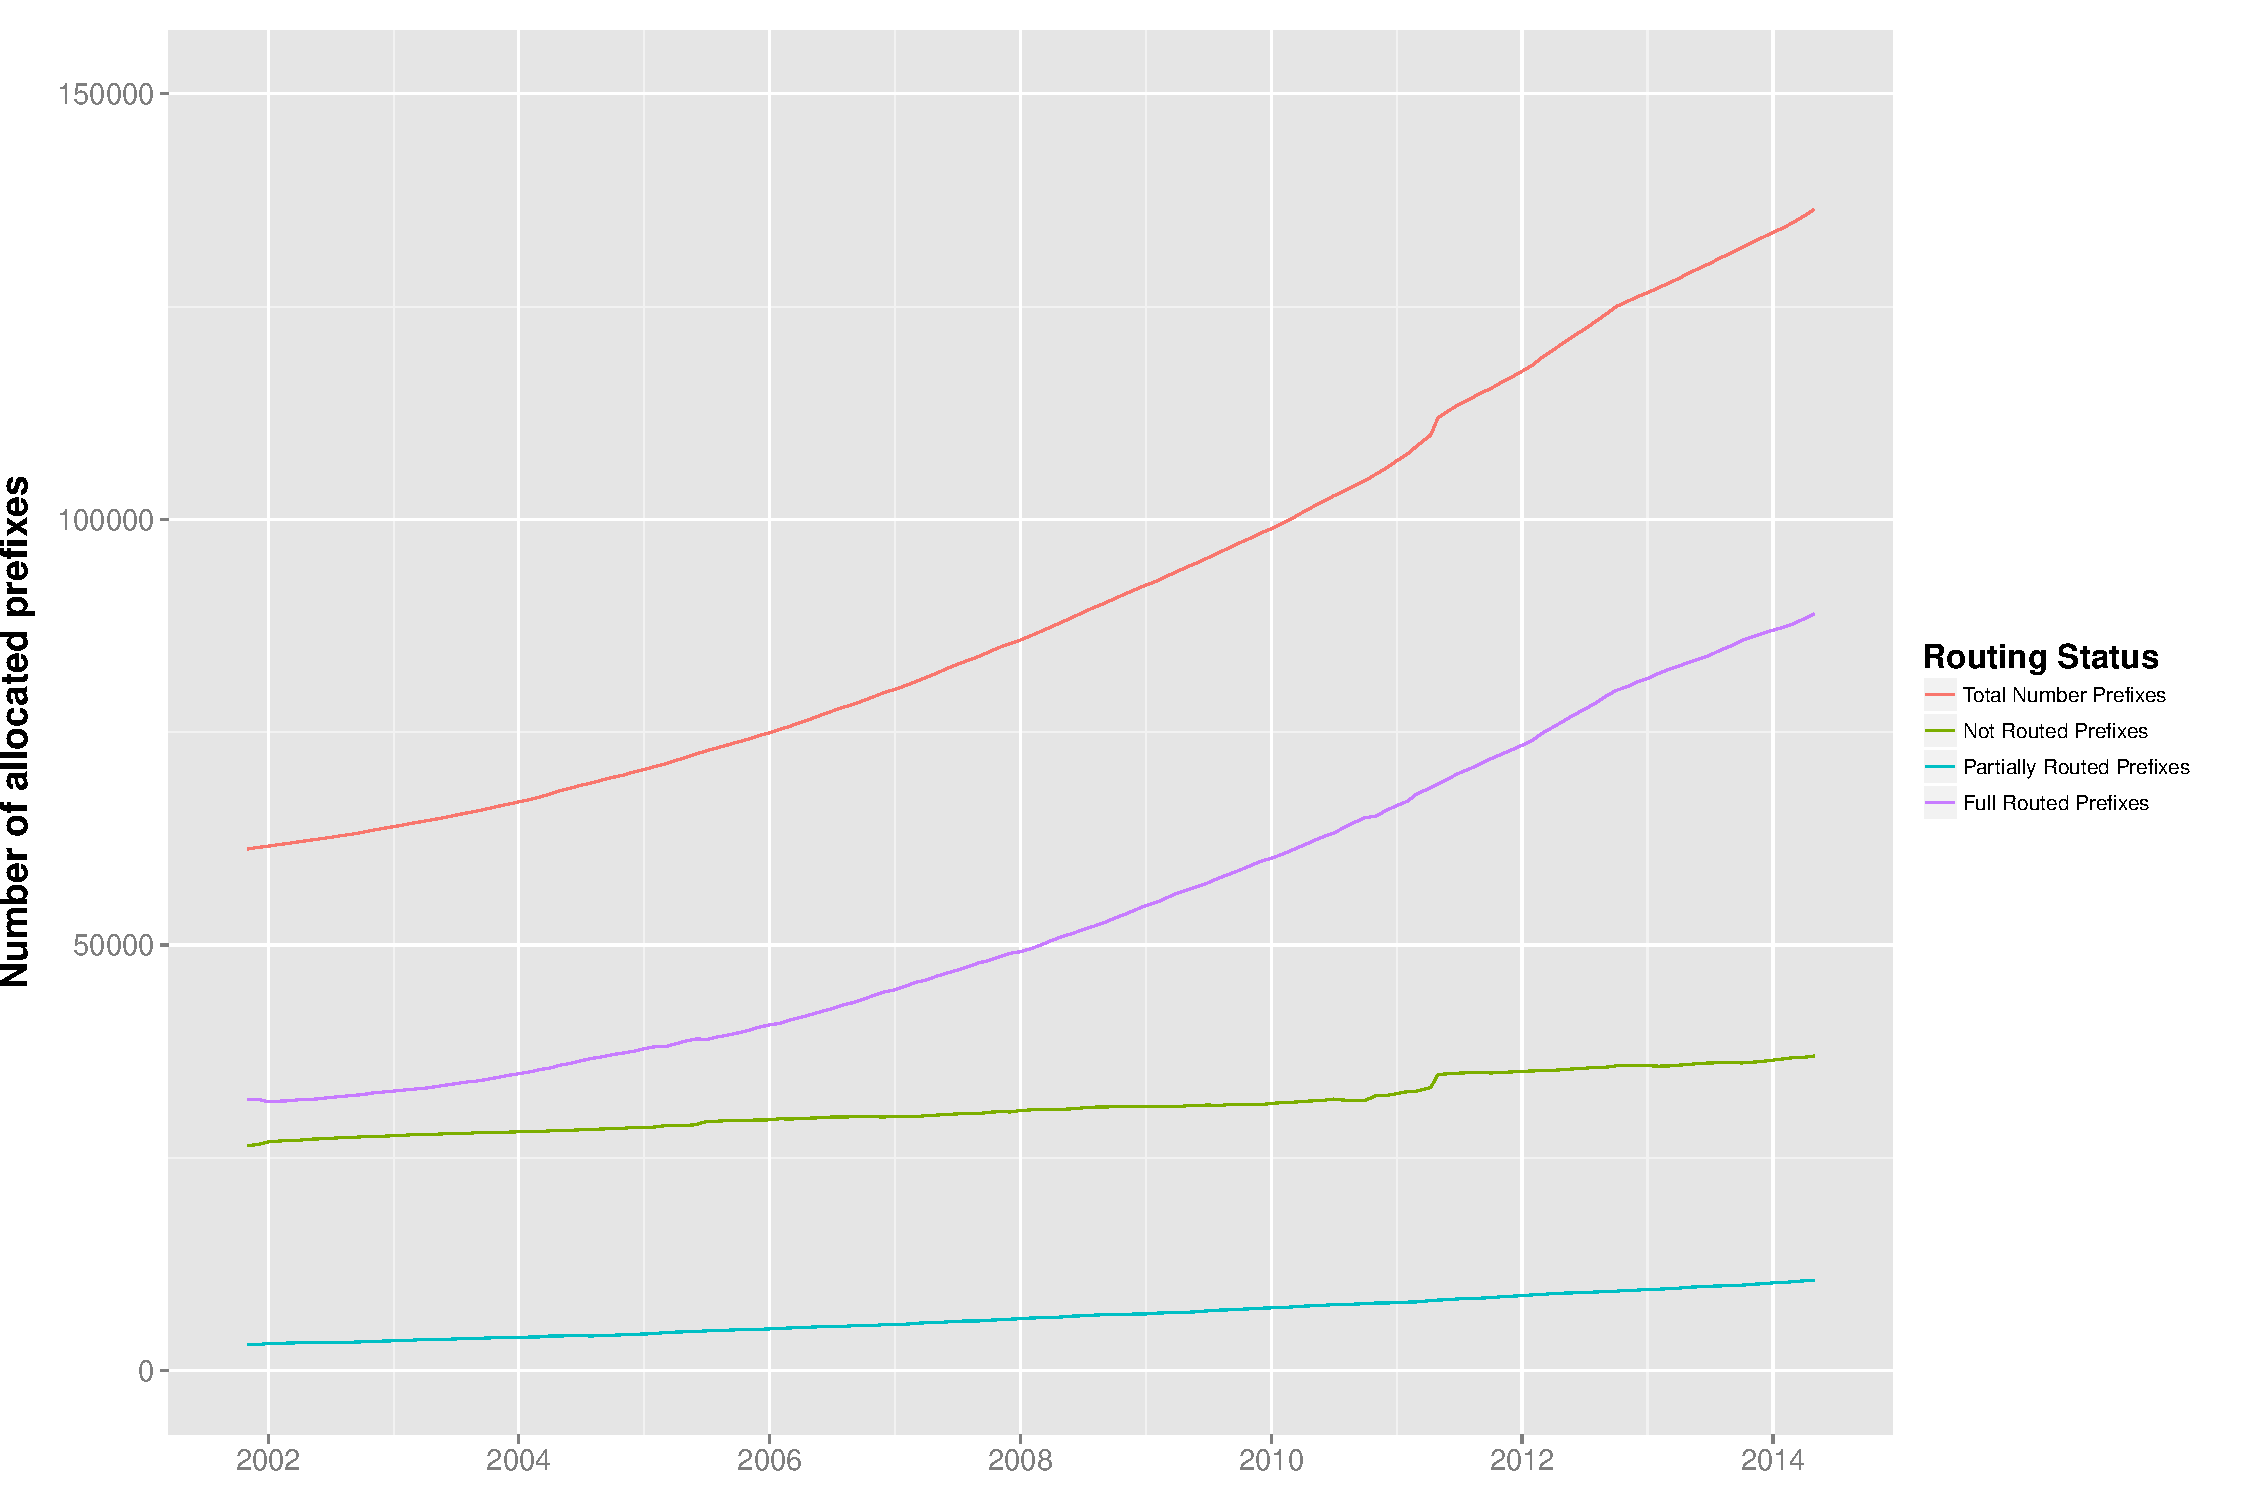
\includegraphics[scale=0.4]{routingStatusGlobal.pdf}
\caption{routingStatusGlobal}
\label{fig:routingStatusGlobal}
\end{figure}

\chapter{Conclusion}
\bibliographystyle{plain}
\renewcommand\bibname{\chapter{References}}
\begin{thebibliography}{count}

\bibitem{Misdirection}
    Rensys Blog,
    \emph{The New Threat: Targeted Internet Traffic Misdirection}.
    [Online]. Available: http://www.renesys.com/2013/11/mitm-internet-hijacking/


\bibitem{Pakistan}
    Rensys Blog,
    \emph{Pakistan Hijacks YouTube}.
    [Online]. Available: http://www.renesys.com/blog/2008/02/pakistan\_hijacks\_
youtube\_1.shtml

\bibitem{Address_Space_Deaggregation}
	L. Cittadini, W. Mühlbauer, S. Uhlig, R. Bush, P. Francois and O.Maennel,
	\emph{Evolution of Internet Address Space Deaggregation: Myths and Reality}.
	IEEE JSAC, Aug 2010.
	
\bibitem{IPv4_Transfer_Markets}
	I. Livadariu, A. Elmokashfi, A. Dhamdhere, Kc Claffy,
	\emph{A First Look at IPv4 Transfer Markets}.
	CoNEXT, 2013.
	
\bibitem{IANA_Address_Space}
	IANA,
	\emph{IANA IPv4 Address Space Registry}.
	[Online]. Available: http://www.iana.org/assignments/ipv4-address-space/ipv4-address-space.xhtml
	
\bibitem{Potaroo}
	G. Huston,
	\emph{IPv4 Address Report}.
	[Online]. Available: http://www.potaroo.net/tools/ipv4/

\bibitem{RouteViews}
	RouteViews,
	\emph{University of Oregon Route Views Project}.
	[Online]. Available: http://www.routeviews.org/
	
\bibitem{Whois}
	Whois,
	\emph{WHOIS Protocol Specification - RFC3912}.
	[Online]. Available: http://tools.ietf.org/html/rfc3912

\bibitem{RADB}
	Whois,
	\emph{Merit RADB - The Routing Assets Database}.
	[Online]. Available: http://www.ra.net/

\bibitem{Impact_Structure_Routing_Tables}
	H. Narayan, R. Govindan, G. Varghese,
	\emph{The Impact of Address Allocation and Routing on the Structure and Implementation of Routing Tables}.
	In Proceedings of the ACM SIGCOMM, 2003.
	
\bibitem{Slowing_Routing_Table_Growth}
	S. Bellovin, R. Bush, T. Griffin, J. Rexford,
	\emph{Slowing routing table growth by filtering based on address allocation policies}.
	June 2001. www.cs.princeton.edu/ jrex.

\bibitem{BGP_Routing_Table_Evolution}
	X. Meng, Z. Xu, B. Zhang, G. Huston, S. Lu, L. Zhang,
	\emph{IPv4 Address Allocation and the BGP Routing Table Evolution}.
	In Proceedings of the ACM SIGCOMM Computer Communication Review, pages 71–80, New York, NY, USA, 2005. ACM Press.

\bibitem{Delegation_Structure}
	A. Sriraman, K.R.B. Butler, P.D. McDaniel, P. Raghavan,
	\emph{Analysis of the IPv4 Address Space Delegation Structure}.
	In IEEE Symposium on Computers and Communications (ISCC), pages 501-508, Jul. 2007.
	
\end{thebibliography}	
\end{document}